\documentclass[portrait,final,a0paper,fontscale=0.25]{baposter}

\usepackage{amsthm, overpic, ae, aecompl, pifont}
\usepackage{amsmath}
\usepackage{amssymb}
\usepackage{relsize}
\usepackage{multirow}
\usepackage{rotating}
\usepackage{bm}
\usepackage{url}
\usepackage{graphics, graphicx}
\usepackage{paralist}
\usepackage{xargs}
\usepackage{xcolor}
\usepackage{ulem}
\usepackage{tikz}\usetikzlibrary{trees,snakes,shapes,arrows,matrix,calc}
\usepackage{shuffle}
\usepackage{hyperref}

\newcommand{\captionfont}{\footnotesize}
\graphicspath{{pictures/}}
\usetikzlibrary{calc}

\newcommand{\blossom}{^\text{\ding{96}}} % blossom

%%%%%%%%%%%%%%%%%%%%%%%%%%%%%%%%%%%%%%%%%%%%%%%%%%%%%%%%%%%%%%%%%%%%%%%%%%%%%%%%
% Some math symbols used in the text
%%%%%%%%%%%%%%%%%%%%%%%%%%%%%%%%%%%%%%%%%%%%%%%%%%%%%%%%%%%%%%%%%%%%%%%%%%%%%%%%

% theorems
\newtheorem*{theorem}{Theo}
\newtheorem*{proposition}{Prop}

\theoremstyle{definition}
\newtheorem*{example}{Exm}
\newtheorem*{remark}{Rmk}

% newcommands
% math special letters
\newcommand{\R}{\mathbb{R}} % reals
\newcommand{\N}{\mathbb{N}} % naturals
\newcommand{\Z}{\mathbb{Z}} % integers
\newcommand{\I}{\mathbb{I}} % set of integers
\newcommand{\C}{\mathbb{C}} % set of summands
\newcommand{\fA}{\mathfrak{A}} % alternating group
\newcommand{\fS}{\mathfrak{S}} % symmetric group
\newcommand{\cC}{\mathcal{C}} % circle
\renewcommand{\b}[1]{\mathbf{#1}} % bold letters

% general math commands
\newcommand{\set}[2]{\left\{ #1 \;\middle|\; #2 \right\}} % set notation
\newcommand{\bigset}[2]{\big\{ #1 \;|\; #2 \big\}} % big set notation
\newcommand{\biggset}[2]{\bigg\{ #1 \;\bigg|\; #2 \bigg\}} % bigg set notation
\newcommand{\ssm}{\smallsetminus} % small set minus
\newcommand{\dotprod}[2]{\langle \, #1 \; | \; #2 \, \rangle} % dot product
\newcommand{\symdif}{\triangle} % symmetric difference
\newcommand{\one}{{1\!\!1}} % the all one vector
\newcommand{\eqdef}{\mbox{\,\raisebox{0.2ex}{\scriptsize\ensuremath{\mathrm:}}\ensuremath{=}\,}} % :=
\newcommand{\defeq}{\mbox{~\ensuremath{=}\raisebox{0.2ex}{\scriptsize\ensuremath{\mathrm:}} }} % =:
\newcommand{\polar}{^\diamond} % polar
\newcommand{\simplex}{\triangle} % simplex
\newcommand{\binomspec}[3]{\begin{pmatrix} #1 \\ #2 \end{pmatrix}_{\!\!#3}} % special binomial coefficient (ou {\begin{Bmatrix} #1 \\ #2 \end{Bmatrix}_{#3})
\renewcommand{\implies}{\Rightarrow} % imply sign

% brick algebra
\newcommandx{\Perm}[2][1=k, 2=n]{\mathsf{Perm}^{#1}(#2)} % permutahedron
\newcommandx{\Brick}[2][1=k, 2=n]{\mathsf{Brick}^{#1}(#2)} % brick polytope
\newcommandx{\SummandBrick}[3][1=k, 2=n, 3=b]{\mathsf{Brick}^{#1}_{#3}(#2)} % summand brick polytope
\newcommandx{\Zono}[2][1=k, 2=n]{\mathsf{Zono}^{#1}(#2)} % zonotope
\newcommand{\signature}{\varepsilon} % signature
\newcommand{\signatures}{\mathcal{E}} % signatures
\newcommand{\up}[1]{\overline{#1}}
\newcommand{\upr}[1]{{\color{red} \overline{#1}}}
\newcommand{\upb}[1]{{\color{blue} \overline{#1}}}
\newcommand{\down}[1]{\underline{#1}}
\newcommand{\downr}[1]{{\color{red} \underline{#1}}}
\newcommand{\downb}[1]{{\color{blue} \underline{#1}}}
\newcommand{\PSymbol}{\mathbf{P}} % P-symbol
\newcommand{\QSymbol}{\mathbf{Q}} % Q-symbol
\newcommandx{\tree}[1][1=T]{\mathrm{#1}} % tree
\DeclareRobustCommand{\verylongrightarrow}{\joinrel\relbar\joinrel\relbar\joinrel\relbar\joinrel\relbar\joinrel\relbar\joinrel\rightarrow}
\newcommandx{\surjectionPermBrick}[1][1=k]{\mathsf{ins}^{#1}} % insertion
\newcommandx{\surjectionBrickZono}[1][1=k]{\mathsf{can}^{#1}} % canopy
\newcommandx{\surjectionPermZono}[1][1=k]{\mathsf{rec}^{#1}} % recoils
\newcommand{\Cone}{\mathrm{C}} % cone
\renewcommand{\b}[1]{\mathbf{#1}} % bold letters
\newcommand{\HH}{\mathbb{H}} % hyperplane
\newcommand{\FQSym}{\mathsf{FQSym}} % quasi-symmetric functions
\newcommand{\CambTrees}{\mathrm{Camb}} % Cambrian trees
\newcommand{\Camb}{\mathsf{Camb}} % Cambrian algebra
\newcommandx{\Twist}[1][1 = k]{\mathsf{Twist}^{#1}} % twist algebra
\newcommand{\PBT}{\mathsf{PBT}} % Loday-Ronco algebra
\newcommand{\Rec}{\mathsf{Rec}} % Solomon algebra
\newcommand{\product}{\cdot} % product
\newcommand{\coproduct}{\triangle} % coproduct
\newcommand{\shiftedShuffle}{\,\bar\shuffle\,} % shifted shuffle
\newcommand{\convolution}{\star} % shifted shuffle
\newcommand{\mirror}[1]{\stackrel{\leftarrow}{#1}} % mirror image of a word
\newcommand{\F}{\mathbb{F}} % F-basis of FQSym
\newcommand{\G}{\mathbb{G}} % G-basis of FQSym
\newcommand{\X}{\mathbb{X}} % X-basis of Rec
\newcommand{\PCamb}{\mathbb{P}} % P-basis of Camb
\newcommand{\QCamb}{\mathbb{Q}} % Q-basis of Camb*
\newcommand{\HCamb}{\mathbb{H}} % H-basis of Camb
\newcommand{\ECamb}{\mathbb{E}} % E-basis of Camb
\newcommand{\PTwist}{\mathbb{P}} % P-basis of Twist
\newcommand{\linearExtensions}{\mathcal{L}} % linear extensions
\newcommand{\Tex}{\includegraphics[scale=2]{Tex}} % example of Cambrian tree
\newcommand{\cB}{\mathcal{B}} % bigebra
\newcommand{\edgecut}[2]{\left( #1 \;\middle\|\; #2 \right)} % edge cut
\newcommand{\Hyp}{\b{H}^=} % hyperplane
\newcommand{\HS}{\b{H}^\ge} % half-space
\newcommandx{\twist}[1][1=T]{\mathrm{#1}} % twist
\newcommandx{\orientation}[1][1=O]{\mathrm{#1}} % orientation
\newcommand{\contact}{^\#} % contact graph
\newcommand{\duality}{^\star} % dual
\newcommand{\projDown}{\pi_\downarrow} % Down projection
\newcommand{\projUp}{\pi^\uparrow} % Down projection
\newcommand{\meet}{\wedge} % meet
\newcommand{\join}{\vee} % join
\newcommandx{\AcyclicTwists}[1][1 = k]{\mathcal{AT}^{#1}} % set of acyclic twists
\newcommandx{\AcyclicOrientations}[1][1 = k]{\mathcal{AO}^{#1}} % set of acyclic orientations
\newcommandx{\Gkn}[2][1=k, 2=n]{\mathrm{G}^{#1}(#2)} % graph k n
\newcommand{\dash}{\,\text{--}\,}
\newcommand{\less}{\vartriangleleft} % smaller WOIP
\newcommandx{\shape}[2][1=k, 2=\signature]{\mathsf{Sh}_{#2}^{#1}} % shape
\newcommand{\underprod}[2]{{#1}\backslash{#2}} % #1 under #2
\newcommand{\overprod}[2]{{#1}\slash{#2}} % #1 over #2
% operators
\DeclareMathOperator{\conv}{conv} % convex hull
\DeclareMathOperator{\cone}{cone} % cone hull
\DeclareMathOperator{\vect}{vect} % linear span
\DeclareMathOperator{\arr}{Arr} % arrangements
\DeclareMathOperator{\inv}{inv} % inversion set

% others
\newcommand{\fref}[1]{Figure~\ref{#1}} % reference figures
\newcommand{\ie}{\textit{i.e.}~} % id est
\newcommand{\eg}{\textit{e.g.}~} % exempli gratia
\newcommand{\vs}{\textit{vs.}~} % versus
\newcommand{\viceversa}{\textit{vice versa}} % vice versa
\newcommand{\ordinal}{\textsuperscript{th}} % th for ordinals
\definecolor{darkblue}{rgb}{0,.1,1} % darkblue color
\newcommand{\darkblue}{\color{darkblue}} % darkblue command
\newcommand{\defn}[1]{\emph{\darkblue #1}} % emphasis of a definition
\renewcommand{\paragraph}[1]{\bigskip\noindent\textbf{#1.}} % paragraph
\setlength{\fboxrule}{1pt}
\newcommand{\colorFrameBox}[2]{{\color{#1}\fbox{\normalcolor#2}}}
\definecolor{red}{rgb}{.95,0,0} % red color
\definecolor{blue}{rgb}{.2,.2,.9} % blue color
\definecolor{green}{rgb}{0,.6,0} % green color
\definecolor{orange}{rgb}{1,.7,0} % orange color

%%%%%%%%%%%%%%%%%%%%%%%%%%%%%%%%%%%%%%%%%%%%%%%%%%%%%%%%%%%%%%%%%%%%%%%%%%%%%%%%
% Fonts
%%%%%%%%%%%%%%%%%%%%%%%%%%%%%%%%%%%%%%%%%%%%%%%%%%%%%%%%%%%%%%%%%%%%%%%%%%%%%%%%

%\usepackage{times}
%\usepackage{helvet}
%\usepackage{bookman}
\usepackage{palatino}

%%%%%%%%%%%%%%%%%%%%%%%%%%%%%%%%%%%%%%%%%%%%%%%%%%%%%%%%%%%%%%%%%%%%%%%%%%%%%%%%
% Multiple bibliographies
%%%%%%%%%%%%%%%%%%%%%%%%%%%%%%%%%%%%%%%%%%%%%%%%%%%%%%%%%%%%%%%%%%%%%%%%%%%%%%%%

\newcommand{\manualBiblio}[1]{\hfill\vspace{-.1cm}{\color{darkblue}\fontsize{8}{10}\selectfont #1}}

%%%%%%%%%%%%%%%%%%%%%%%%%%%%%%%%%%%%%%%%%%%%%%%%%%%%%%%%%%%%%%%%%%%%%%%%%%%%%%%%
% Multicol Settings
%%%%%%%%%%%%%%%%%%%%%%%%%%%%%%%%%%%%%%%%%%%%%%%%%%%%%%%%%%%%%%%%%%%%%%%%%%%%%%%%
\makeatletter
\renewcommand{\baposter@columns}{6}%
\makeatother

\setlength{\columnsep}{1.5em}
\setlength{\columnseprule}{0mm}

%%%%%%%%%%%%%%%%%%%%%%%%%%%%%%%%%%%%%%%%%%%%%%%%%%%%%%%%%%%%%%%%%%%%%%%%%%%%%%%%
% Save space in lists and displayed formulas.
%%%%%%%%%%%%%%%%%%%%%%%%%%%%%%%%%%%%%%%%%%%%%%%%%%%%%%%%%%%%%%%%%%%%%%%%%%%%%%%%
% Use this after the opening of the list
\newcommand{\compresslist}{%
\setlength{\itemsep}{7pt}%
\setlength{\parskip}{-7pt}%
\setlength{\parsep}{0pt}%
\setlength{\topsep}{-2pt}%
}

\makeatletter
\g@addto@macro\normalsize{\setlength\abovedisplayskip{3pt}}
\g@addto@macro\normalsize{\setlength\belowdisplayskip{3pt}}
\makeatother

%%%%%%%%%%%%%%%%%%%%%%%%%%%%%%%%%%%%%%%%%%%%%%%%%%%%%%%%%%%%%%%%%%%%%%%%%%%%%%
%%% Begin of Document
%%%%%%%%%%%%%%%%%%%%%%%%%%%%%%%%%%%%%%%%%%%%%%%%%%%%%%%%%%%%%%%%%%%%%%%%%%%%%%

\begin{document}

%%%%%%%%%%%%%%%%%%%%%%%%%%%%%%%%%%%%%%%%%%%%%%%%%%%%%%%%%%%%%%%%%%%%%%%%%%%%%%
%%% Here starts the poster
%%%---------------------------------------------------------------------------
%%% Format it to your taste with the options
%%%%%%%%%%%%%%%%%%%%%%%%%%%%%%%%%%%%%%%%%%%%%%%%%%%%%%%%%%%%%%%%%%%%%%%%%%%%%%
% Define some colors

\begin{poster}%
  % Poster Options
  {
  % Show grid to help with alignment
  grid=false,
  % Column spacing
  colspacing=.7em,
  % Color style
  bgColorOne=white,
  bgColorTwo=white,
  borderColor=blue,
  headerColorOne=blue,
  headerColorTwo=white,
  headerFontColor=white,
  boxColorOne=white,
  boxColorTwo=green,
  % Format of textbox
  textborder=roundedleft,
  % Format of text header
  eyecatcher=true,
  headerborder=closed,
  headerheight=0.05\textheight,
  textfont=\Huge,
  headershape=roundedright,
  headershade=plain,
  headerfont=\Large\bf, %Sans Serif
  textfont={\setlength{\parindent}{0pt}},
  boxshade=plain,
%  background=shade-tb,
  background=plain,
  linewidth=1pt
  }
  % Eye Catcher
  {Toto}
  % Title
  {{\fontsize{24}{25}\selectfont {\color{green} Non-kissing} \; --- \; {\color{red} vs} \; --- \; {\color{blue} Non-crossing}} \\ {\Large \rm Yann Palu} {\normalsize (UPJV) jtw} {\Large \rm Vincent Pilaud} {\normalsize (LIX, CNRS) and} {\Large \rm Pierre-Guy Plamondon} {\normalsize (Orsay)} \vspace*{-.5cm}}
  % Authors
  {}
  % University logo
  {}
  
%%%%%%%%%%%%%%%%%%%%%%%%%%%%%%%%%%%%%%%%%%%%%%%%%%%%%%%%%%%%%%%%%%%%%%%%%%%%%%
%%% Now define the boxes that make up the poster
%%%---------------------------------------------------------------------------
%%% Each box has a name and can be placed absolutely or relatively.
%%% The only inconvenience is that you can only specify a relative position 
%%% towards an already declared box. So if you have a box attached to the 
%%% bottom, one to the top and a third one which should be in between, you 
%%% have to specify the top and bottom boxes before you specify the middle 
%%% box.
%%%%%%%%%%%%%%%%%%%%%%%%%%%%%%%%%%%%%%%%%%%%%%%%%%%%%%%%%%%%%%%%%%%%%%%%%%%%%%

%%%%%%%%%%%%%%%%%%%%%%%%%%%%%%%%%%%%%%%%%%%%%%%%%%%%%%%%%%%%%%%%%%%%%%%%%%%%%%
\headerbox{From walks on a grid [McConville]...}{name=walks,column=0,span=3,row=0,borderColor=green,headerColorOne=green}{
%%%%%%%%%%%%%%%%%%%%%%%%%%%%%%%%%%%%%%%%%%%%%%%%%%%%%%%%%%%%%%%%%%%%%%%%%%%%%%

\hspace*{.1cm}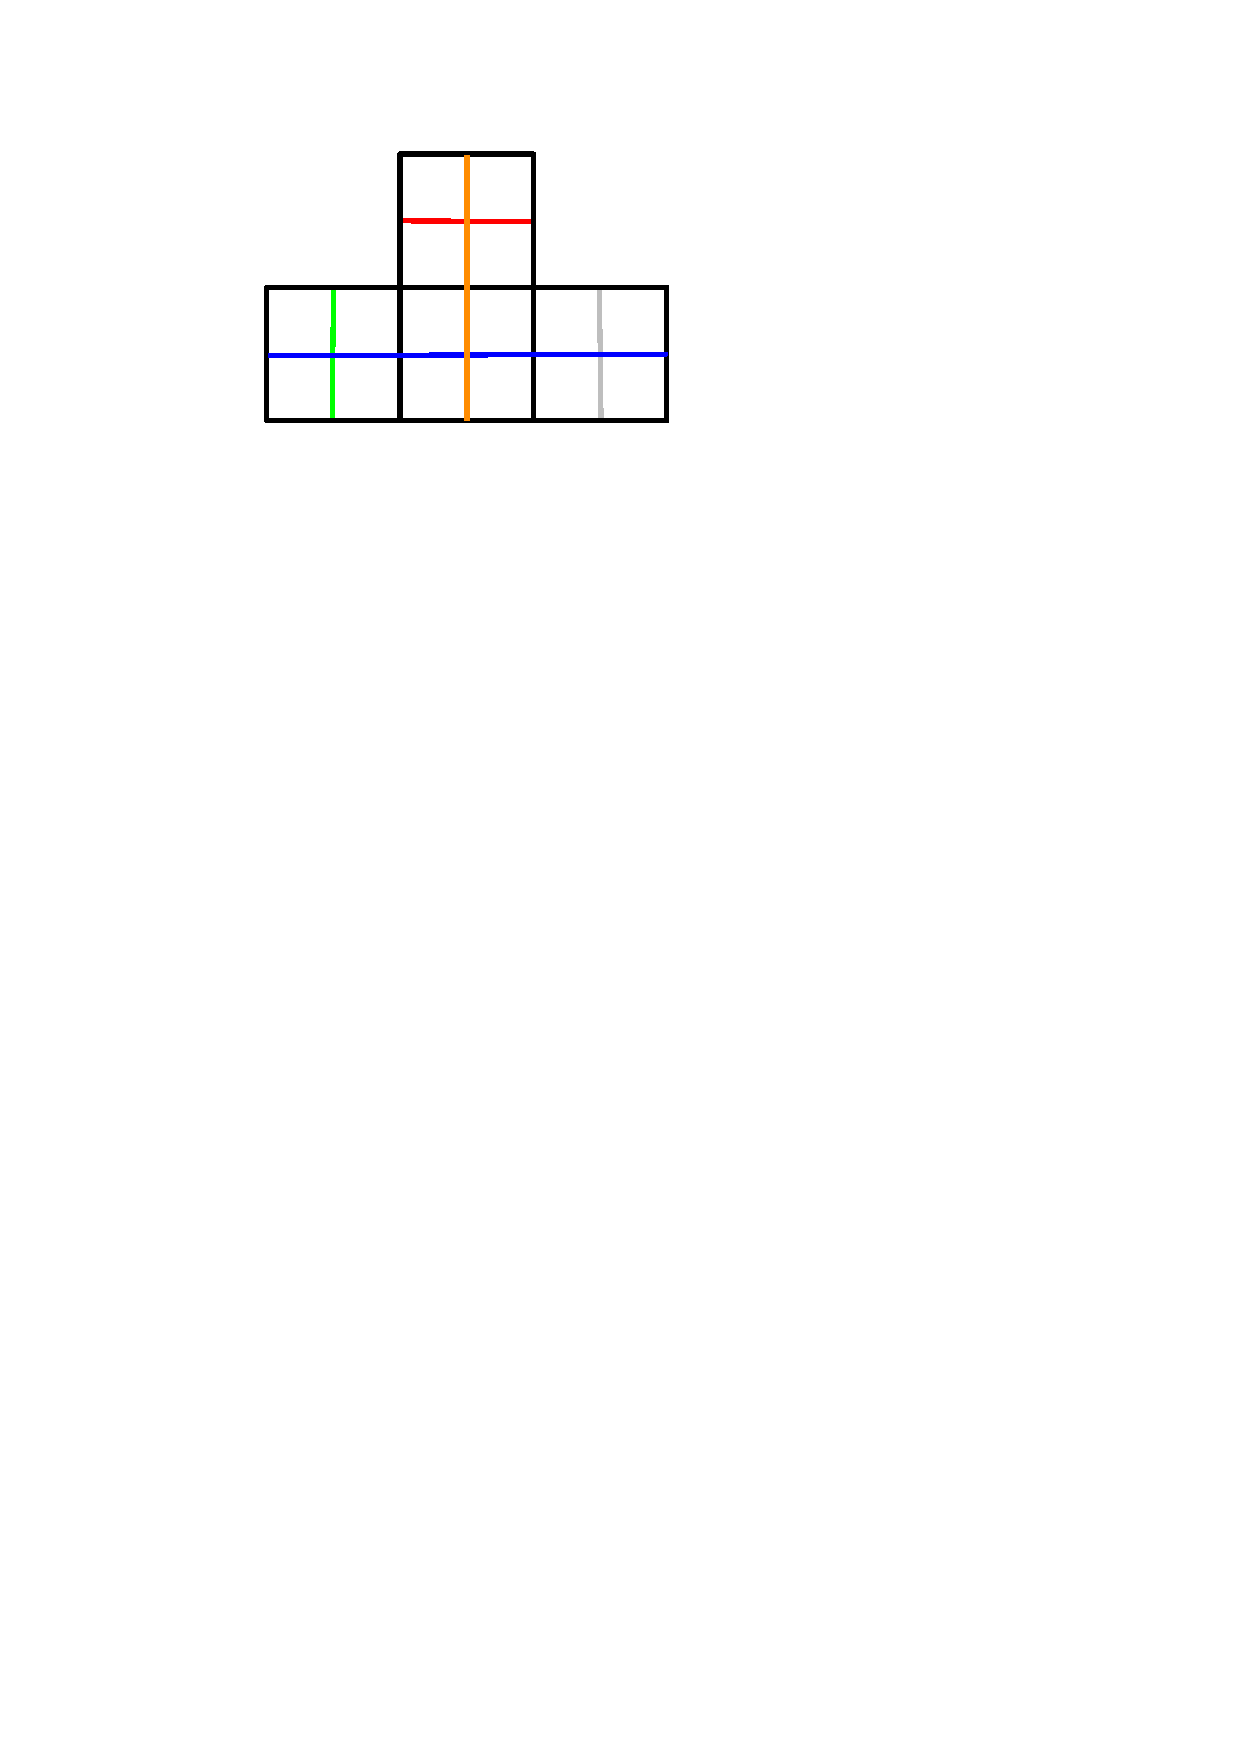
\includegraphics[scale=.3]{StraightWalks}
\hspace*{.3cm}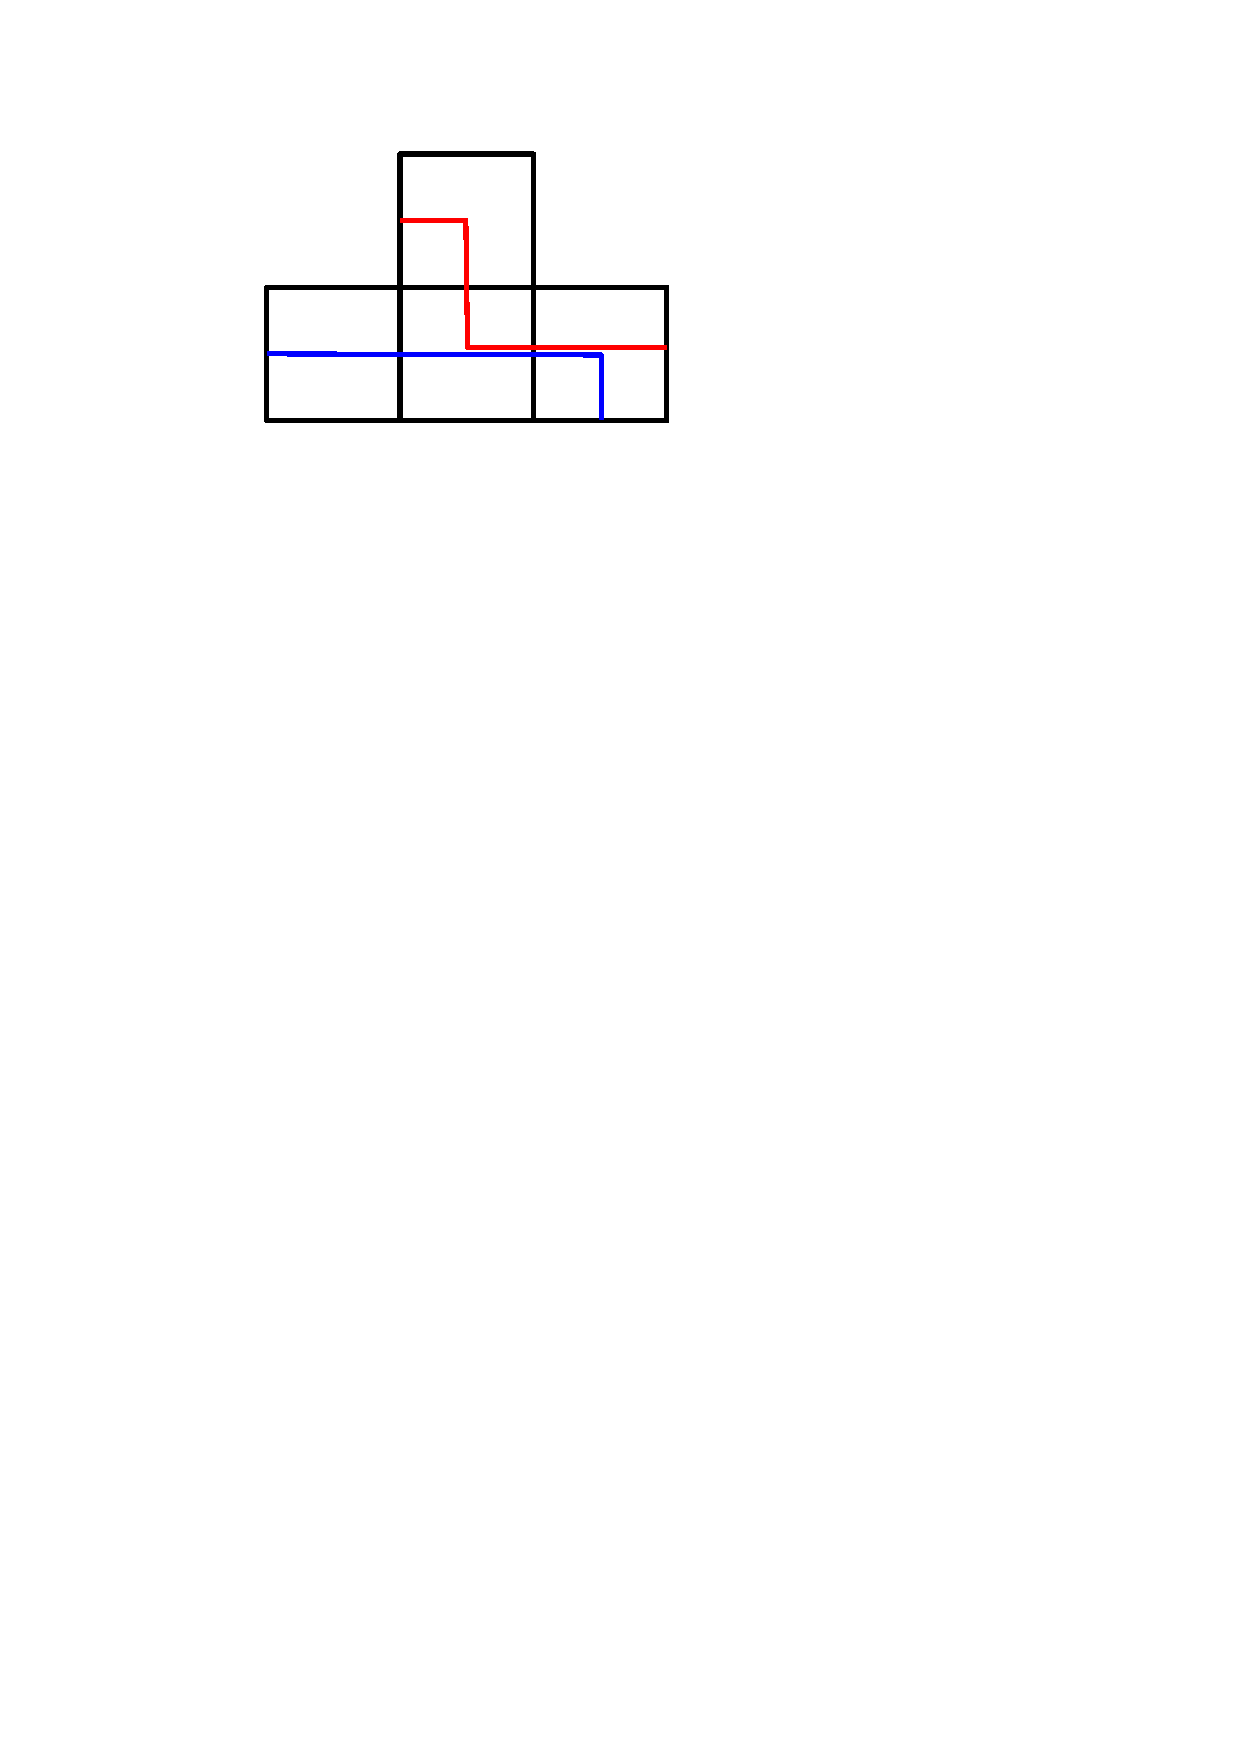
\includegraphics[scale=.3]{Kiss}
\hspace*{.3cm}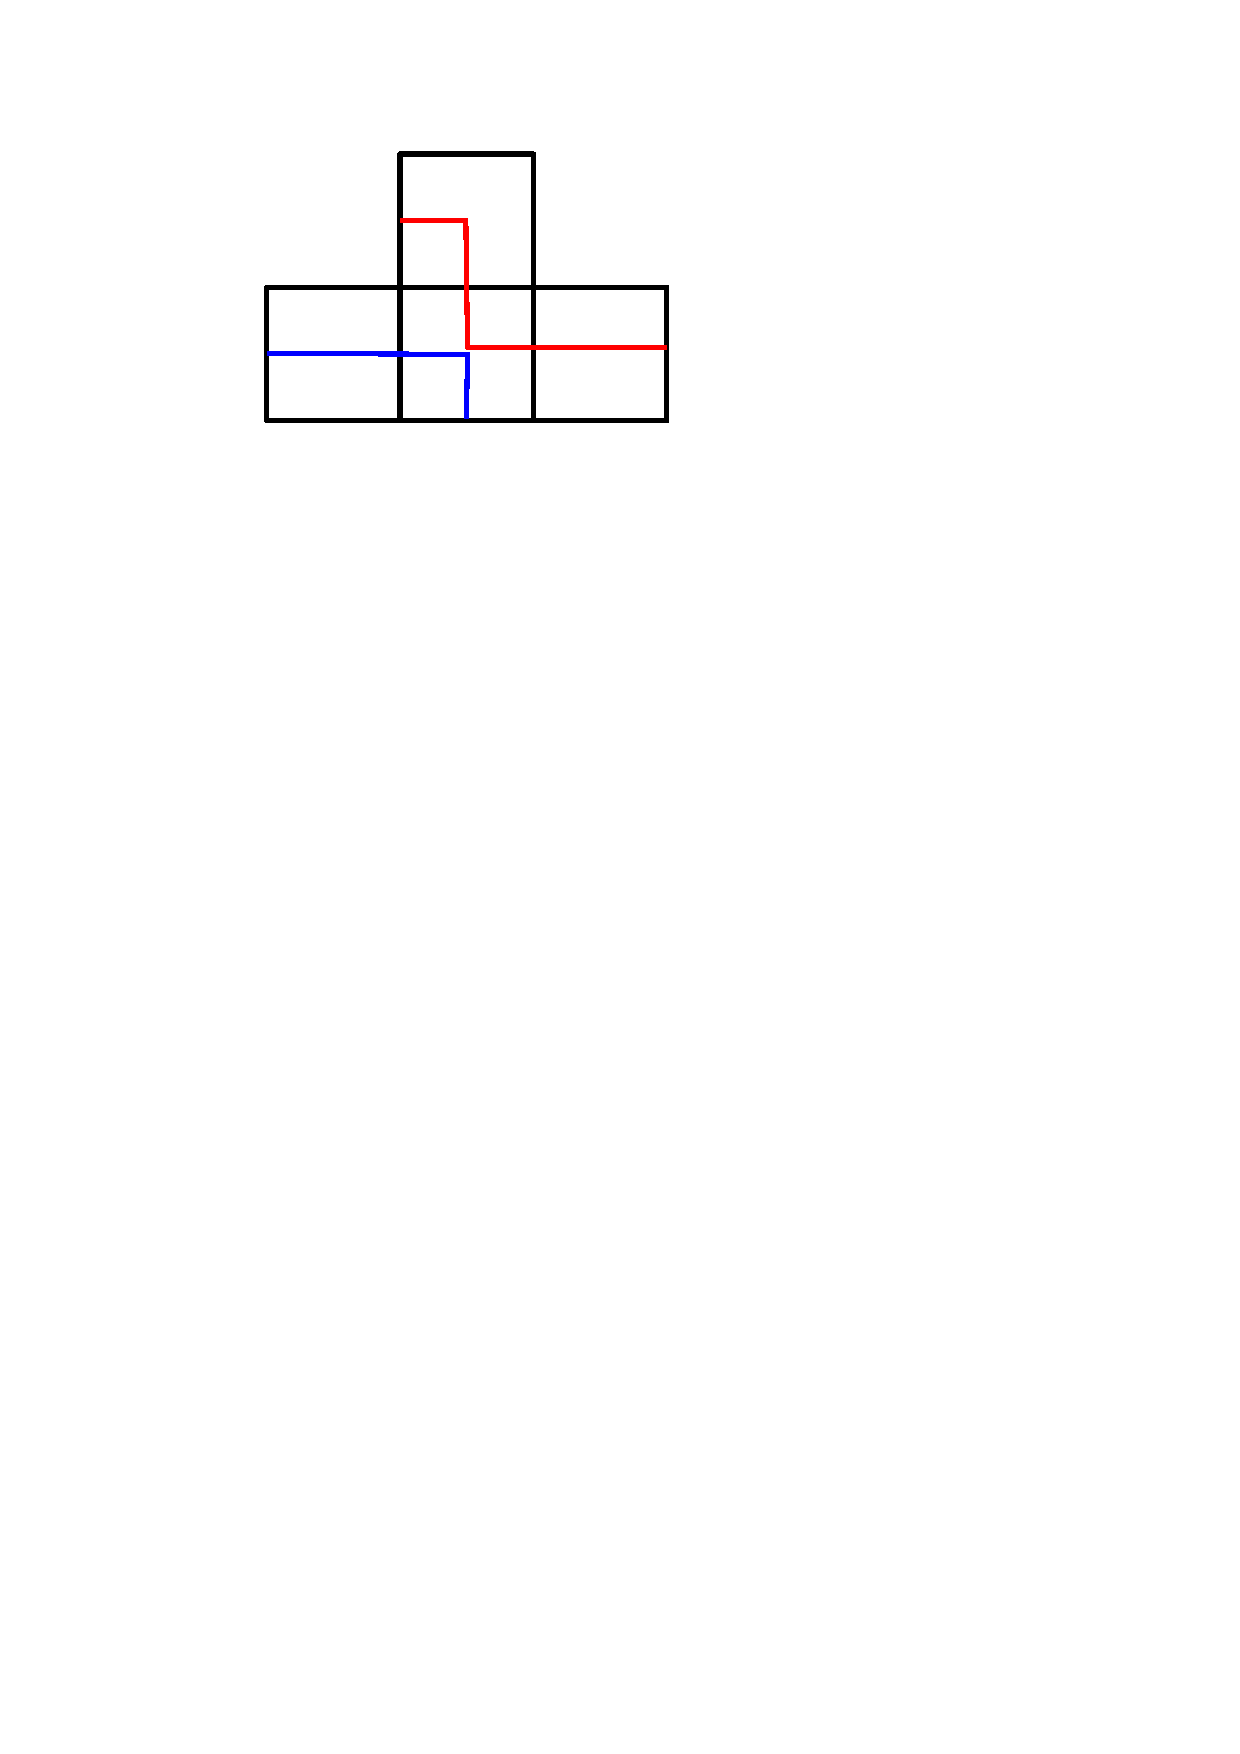
\includegraphics[scale=.3]{ShyKiss}
\hspace*{.3cm}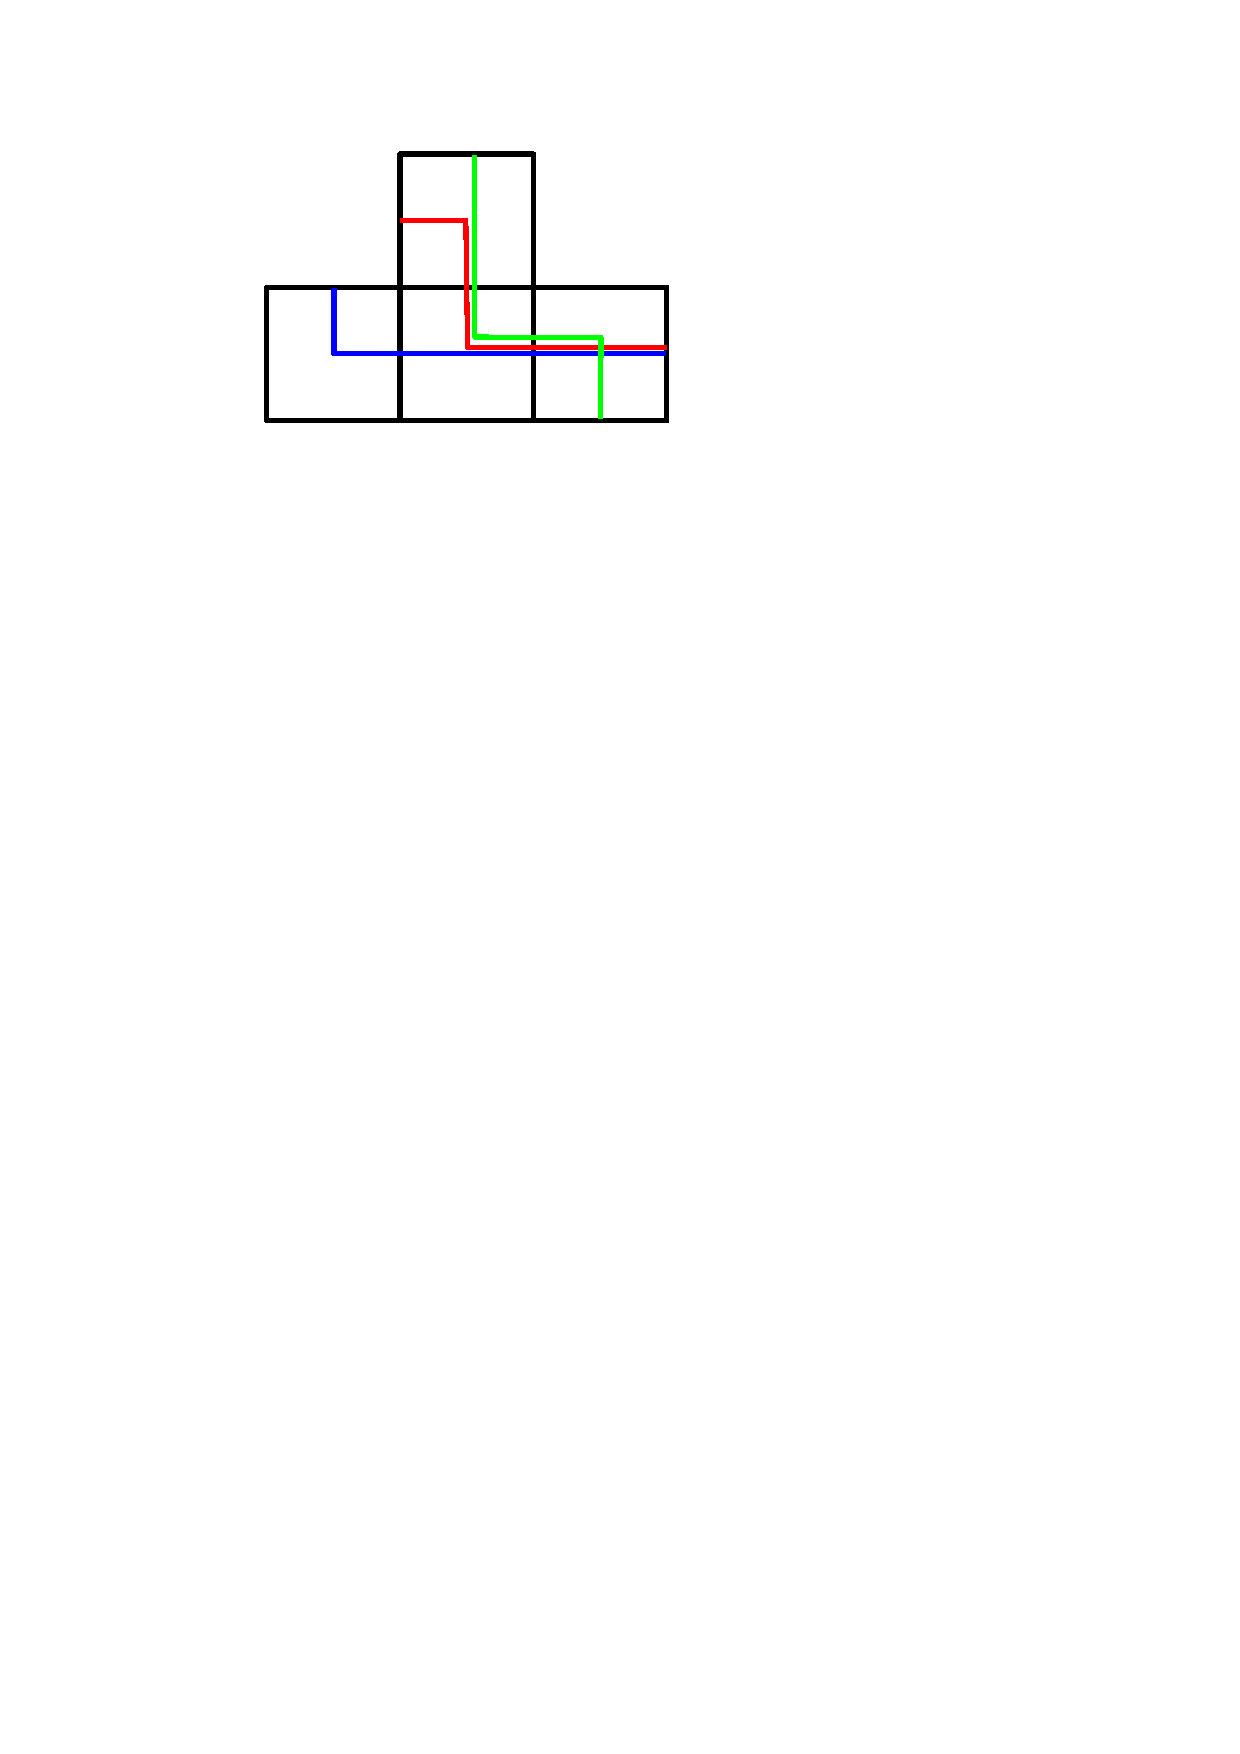
\includegraphics[scale=.3]{NotAKiss}

{\footnotesize The straight walks}
\hspace*{.8cm}{\footnotesize A kiss}
\hspace*{1.3cm}{\footnotesize A shy kiss}
\hspace*{1.1cm}{\footnotesize No kissing}



\vspace{-.2cm}
\hspace{-.25cm}
{\color{green} \rule{10.02cm}{1pt}}
\vspace{-.35cm}

% \begin{minipage}{9.5cm}
{\color{green} walk} $=$ NW to SE maximal walks in a grid of any (fixed) given shape %\\[.2cm]

\medskip

A walk $\omega$ {\color{green} kisses} a walk $\omega'$ if 
\begin{compactitem}
\item $\omega$ and $\omega'$ share a common subpath $\rho$ and
\item $\omega$ enters $\rho$ from W and leaves it towards S while
\item $\omega'$ enters $\rho$ from N and leaves it towards E.
\end{compactitem}
% \end{minipage}

% \vspace{-.2cm}
\hspace{-.25cm}
{\color{green} \rule{10.02cm}{1pt}}
\vspace{-.35cm}

% \begin{minipage}{9.5cm}
{\color{green} (reduced) non-kissing complex} $=$ clique complex of (non-straight) walks for the compatibility relation of non-kissing.

% \end{minipage}
\medskip
{\color{green} \bf Thm} [McC]: {\it The reduced non-kissing complex is pure and thin.}

% 
% {\color{red} Insertion algorithm} \\
% \hspace*{.2cm} surjection~$\surjectionPermBrick$: permutations of~$[n]$ $\longrightarrow$ acyclic $(k,n)$-twists \\
% \hspace*{.2cm} algo: insert pipes from right to left {\color{red} as northwest as possible} \\[.05cm]
% % %\centerline{\includegraphics[width=\textwidth]{insertion}}
% % \centerline{\includegraphics[width=\textwidth]{insertionBis}}
% % %\centerline{\includegraphics[width=.7\textwidth]{insertion1}}
% % %\centerline{\includegraphics[width=.7\textwidth]{insertion2}}
% \hspace*{8cm}
% {\footnotesize $\surjectionPermBrick[2](31542)$}
% 
% \vspace{-.2cm}
% {\color{red} $k$-twist congruence} $=$ transitive closure of \\
% \centerline{$U ac V_1 b_1 V_2 b_2 \cdots V_k b_k W \equiv^k U ca V_1 b_1 V_2 b_2 \cdots V_k b_k W$} \\
% where~$a < b_i < c$ for all $i \in [k]$
% 
% \medskip
% {\color{red} \textsc{prop.}} $\tau \! \equiv^k \!\! \tau'$ $\iff$ $\surjectionPermBrick(\tau) \! = \! \surjectionPermBrick(\tau') \! = \! \twist$ $\iff$ $\tau,\tau' \! \in \! \linearExtensions(\twist\contact)$
% 
% \vspace{-.1cm}
% \hspace{-.25cm}
% {\color{green} \rule{10.02cm}{1pt}}
% \vspace{-.4cm}
% 
% \hspace{5.7cm}
% % 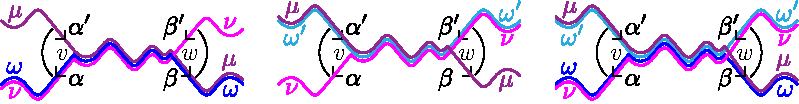
\includegraphics[scale=.65]{flip1} \hspace{-.5cm} \raisebox{.6cm}{$\longrightarrow$} \hspace{.1cm} 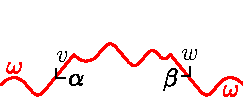
\includegraphics[scale=.65]{flip2}
% 
% \vspace{-1.5cm}
% \begin{minipage}{6cm}
% {\color{red} Flip} $=$ exchange an elbow with \\ its corresponding crossing \\
% {\color{red} Increasing} flip $=$ elbow SE crossing
% \end{minipage}
% 
% \vspace{.2cm}

}

%%%%%%%%%%%%%%%%%%%%%%%%%%%%%%%%%%%%%%%%%%%%%%%%%%%%%%%%%%%%%%%%%%%%%%%%%%%%%%
\headerbox{...to walks on a gentle bound quiver [PPP]}{name=PPP1,column=3,span=3,row=0,borderColor=green,headerColorOne=green}{
%%%%%%%%%%%%%%%%%%%%%%%%%%%%%%%%%%%%%%%%%%%%%%%%%%%%%%%%%%%%%%%%%%%%%%%%%%%%%%

\vspace*{.15cm}\hspace*{7.5cm}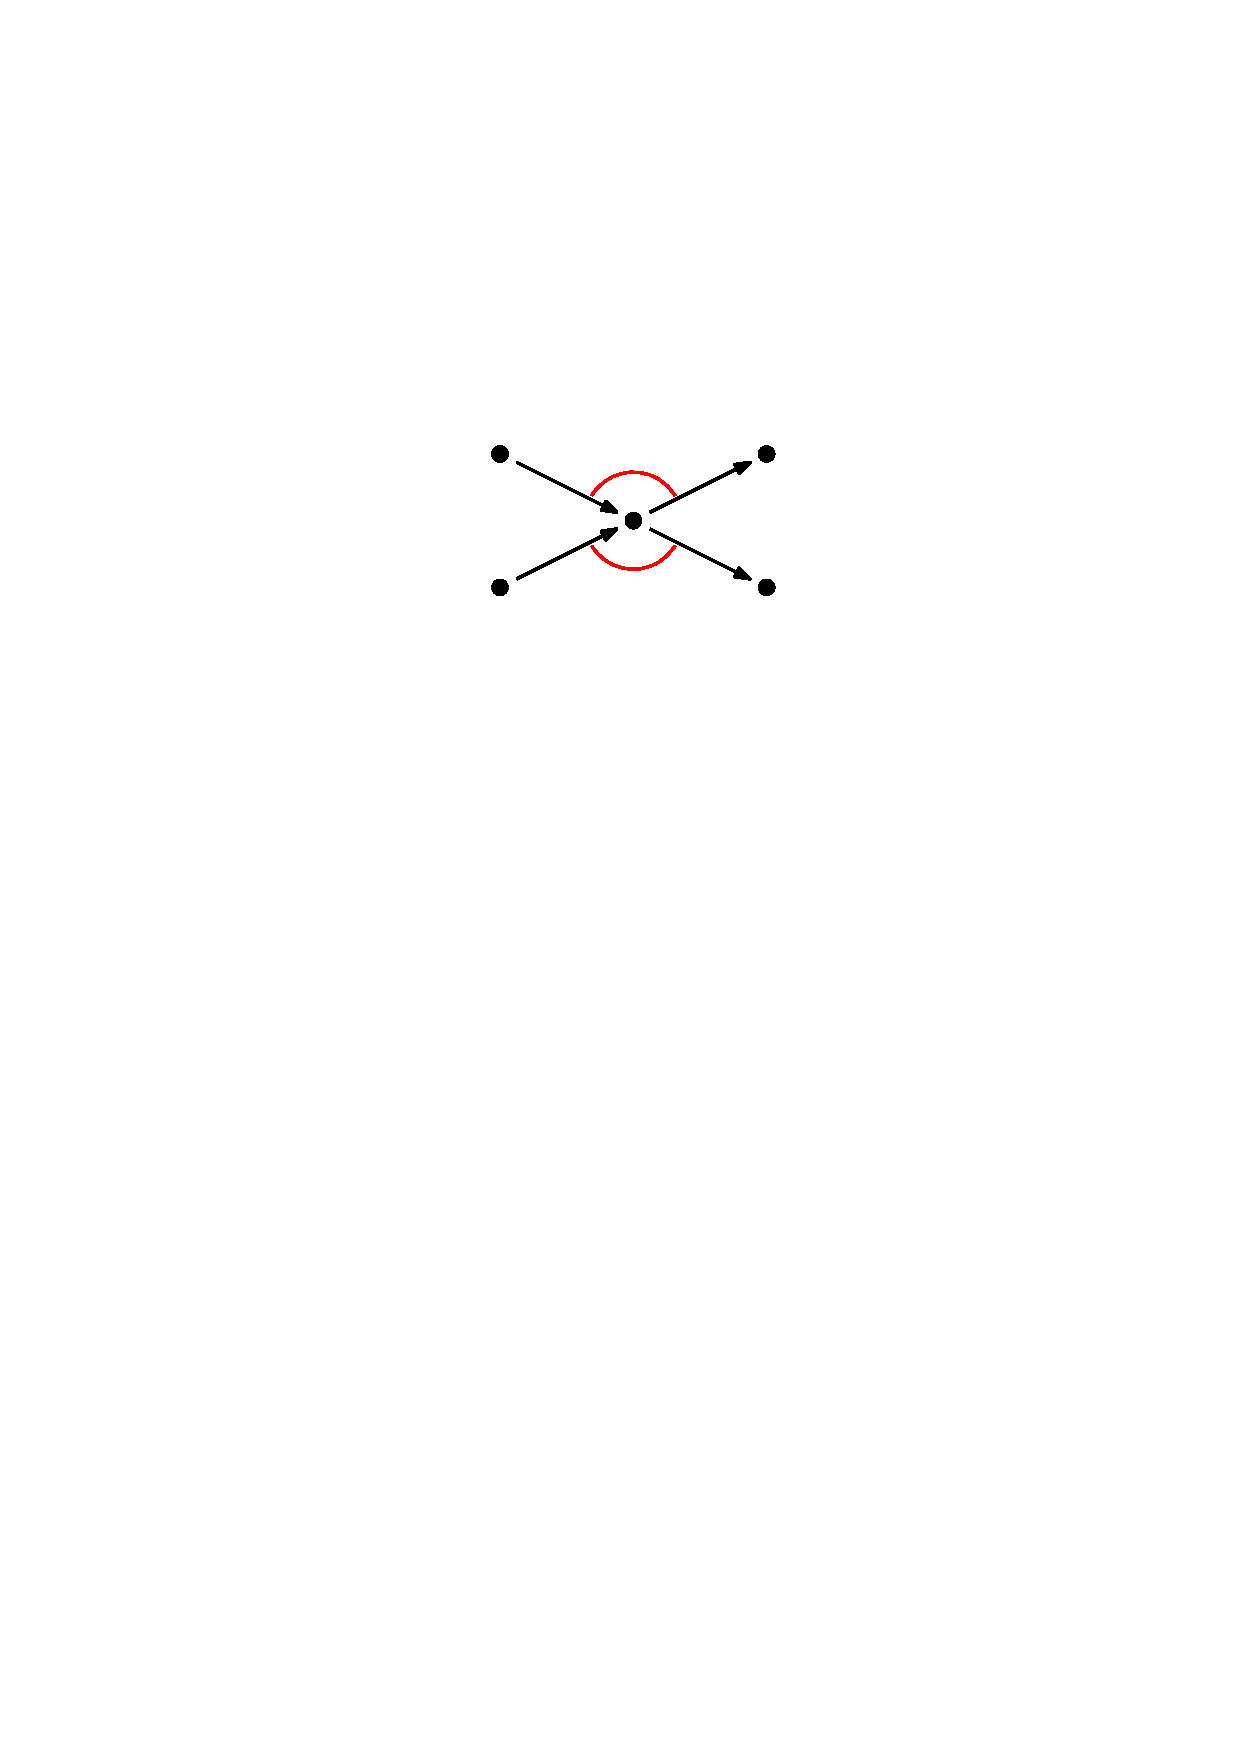
\includegraphics[scale=.35]{GentleCondition}

\vspace*{-1.2cm}
\begin{minipage}{7.2cm}
{\color{green} Gentle bound quiver} $Q =$ oriented graph with relations (forbidden paths) of lenght 2; obtained by glueings of the local configuration:
Moreover, any vertex must have out-degree at most 2 and in-degree at most 2.
%  \item For any arrow $\alpha$, there is at most one arrow $\beta$ such that $\alpha\beta$ (resp. $\beta\alpha$) is not a relation and at most one arrow $\gamma$ such that $\alpha\gamma$ (resp. $\gamma\alpha$) is a relation.
% \end{compactitem}

\medskip

Its {\color{green} Blossoming bound quiver} $Q\blossom$ is obtained by making each (old) vertex 4-valent:
\end{minipage}

\vspace*{-1.9cm}\hspace*{7.5cm}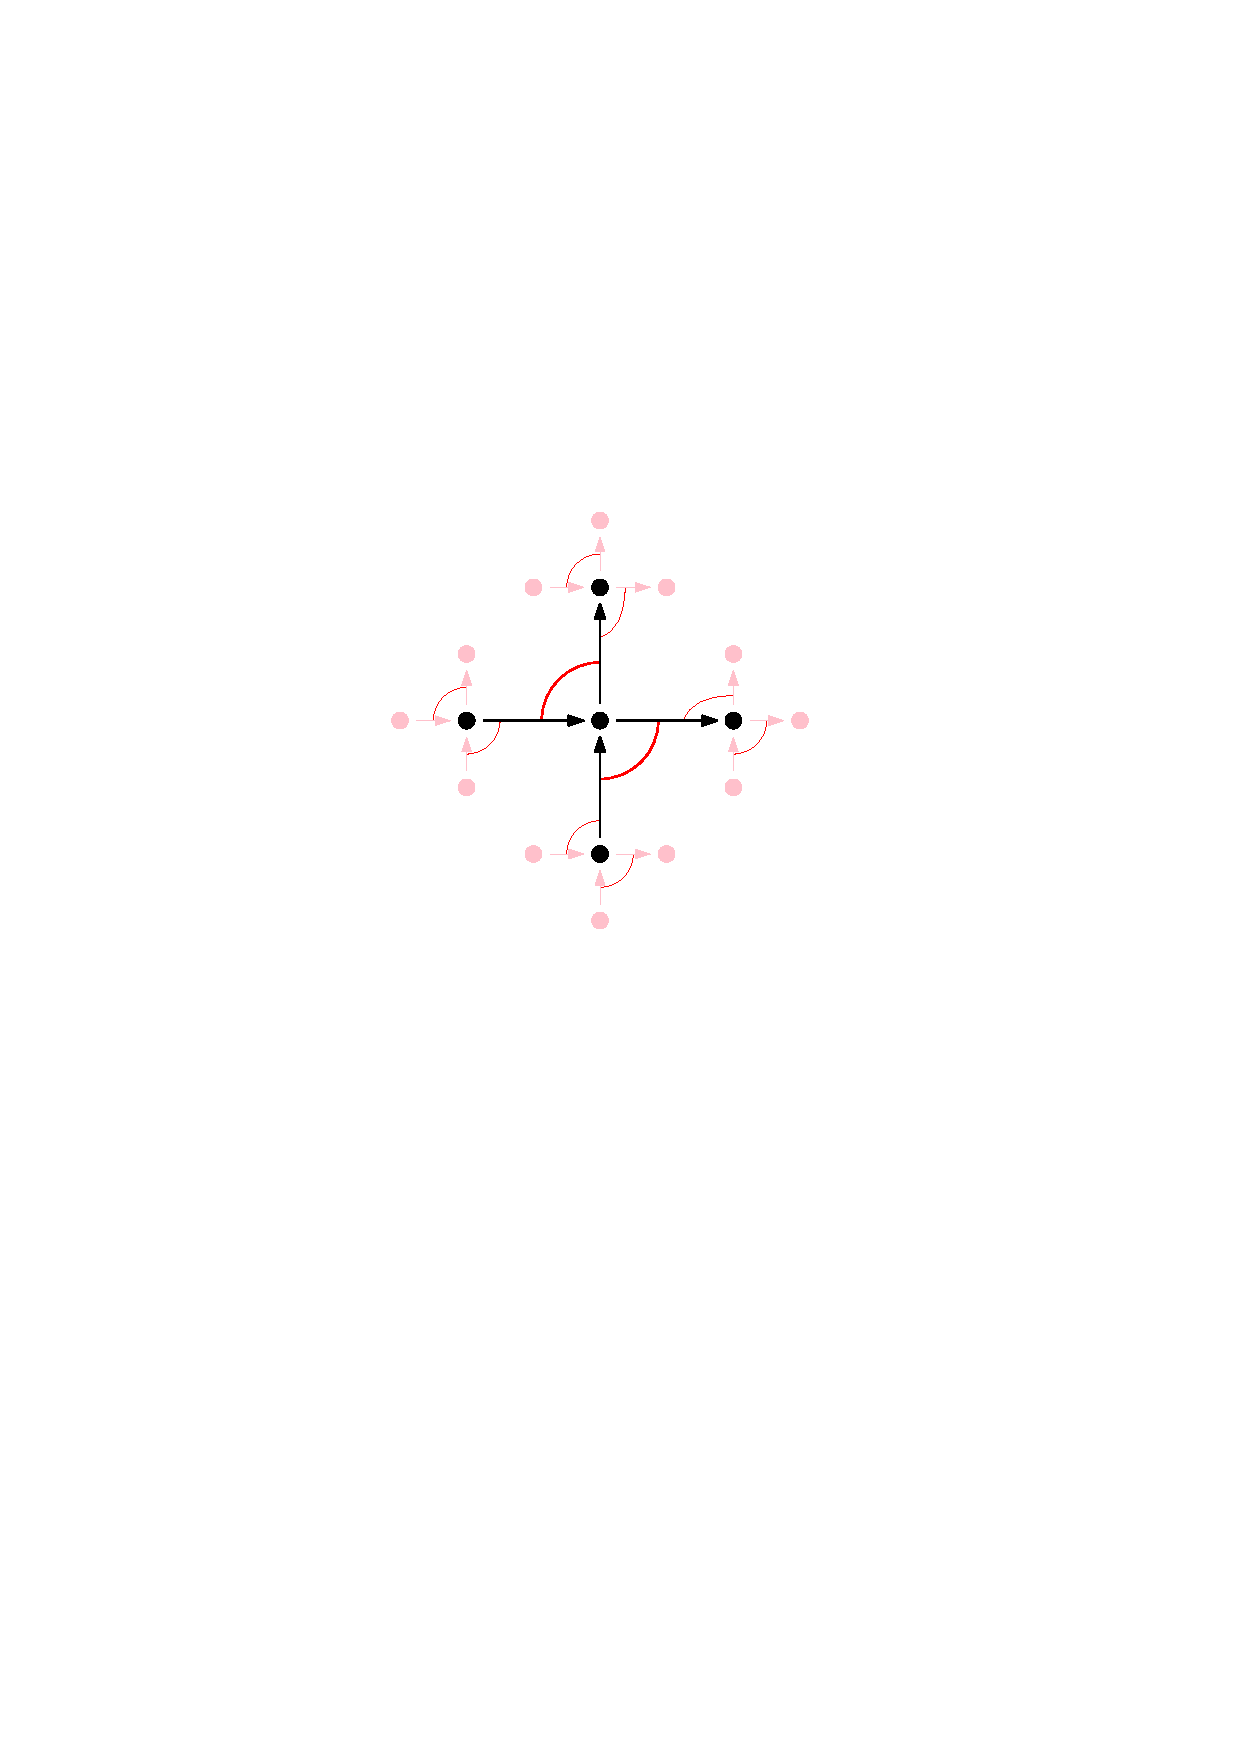
\includegraphics[scale=.3]{BlossomingQuiverGentle}

\vspace{-.35cm}
\hspace{-.25cm}
{\color{green} \rule{10.02cm}{1pt}}
\vspace{-.35cm}

A {\color{green} string} of $Q$ is a word on arrows and their inverses not containing any $\alpha\alpha^{-1}$, $\alpha^{-1}\alpha$ nor any $\alpha\beta$, $\beta^{-1}\alpha^{-1}$ if $\alpha\beta$ is a relation.

\medskip

A {\color{green} walk} on $Q$ is a maximal string of $Q\blossom$.

\vspace*{-.6cm}\hspace*{6cm}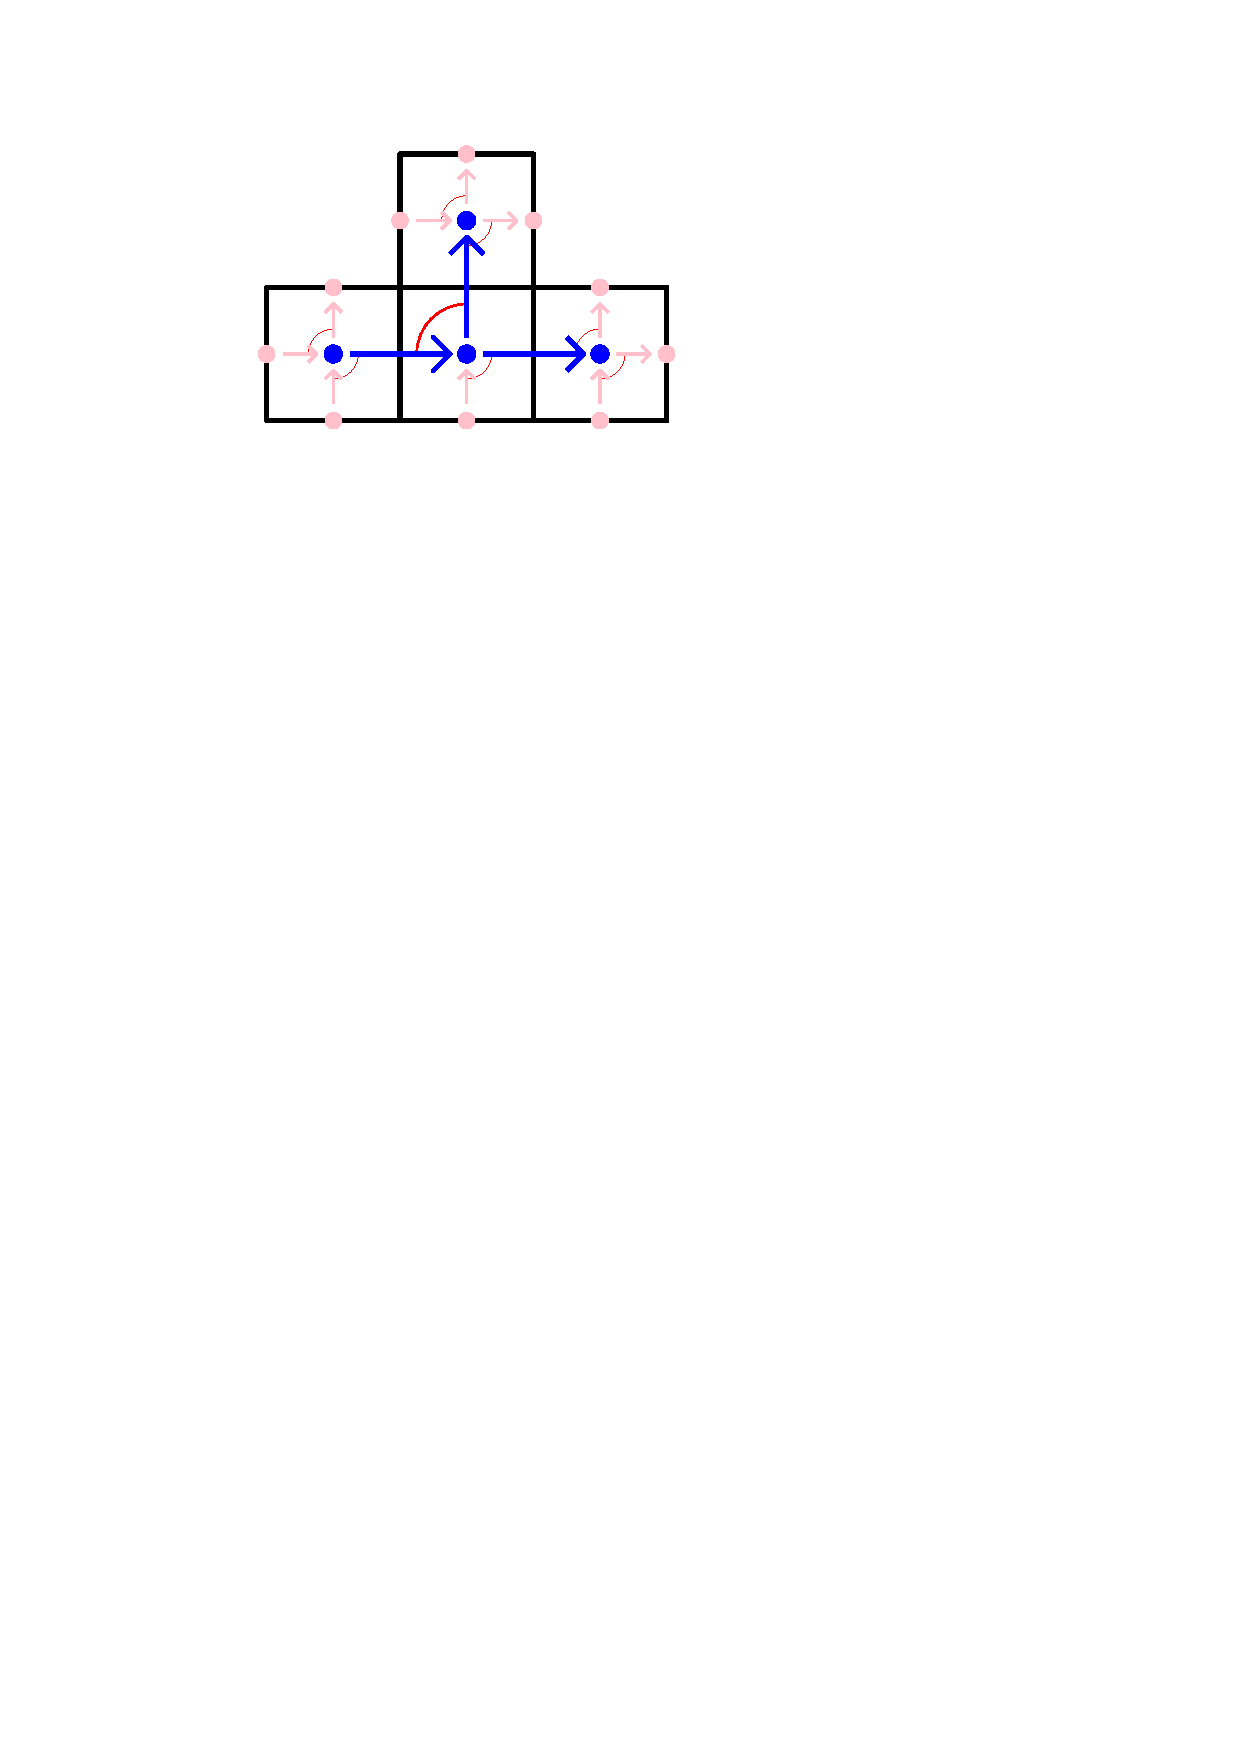
\includegraphics[scale=.4]{BlossomingQuiverGrid}

\vspace*{-1cm}
\begin{minipage}{5.5cm}
 The gentle bound quiver of a grid, and its blossoming: 
\end{minipage}

\vspace{.15cm}
\hspace{-.25cm}
{\color{green} \rule{10.02cm}{1pt}}
\vspace{-.35cm}

% \end{minipage}
\medskip
{\color{green} \bf Thm} [PPP]: {\it The reduced non-kissing complex of any gentle bound} 
\hspace*{1.95cm}{\it quiver is pure and thin.}

\hspace*{3cm}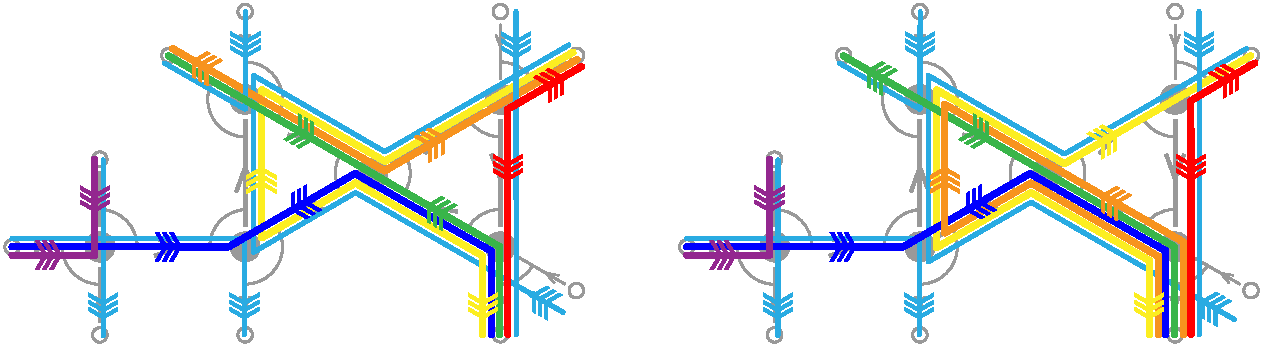
\includegraphics[scale=.3]{exmFlip}

\vspace*{-1.5cm} Example of a flip:
\vspace{.9cm}
}


%%%%%%%%%%%%%%%%%%%%%%%%%%%%%%%%%%%%%%%%%%%%%%%%%%%%%%%%%%%%%%%%%%%%%%%%%%%%%%
\headerbox{From accordions on a disk...[Garver--McC]}{name=accordions,column=0,span=3,below=walks,borderColor=blue,headerColorOne=blue}{
%%%%%%%%%%%%%%%%%%%%%%%%%%%%%%%%%%%%%%%%%%%%%%%%%%%%%%%%%%%%%%%%%%%%%%%%%%%%%%

\hspace*{6cm}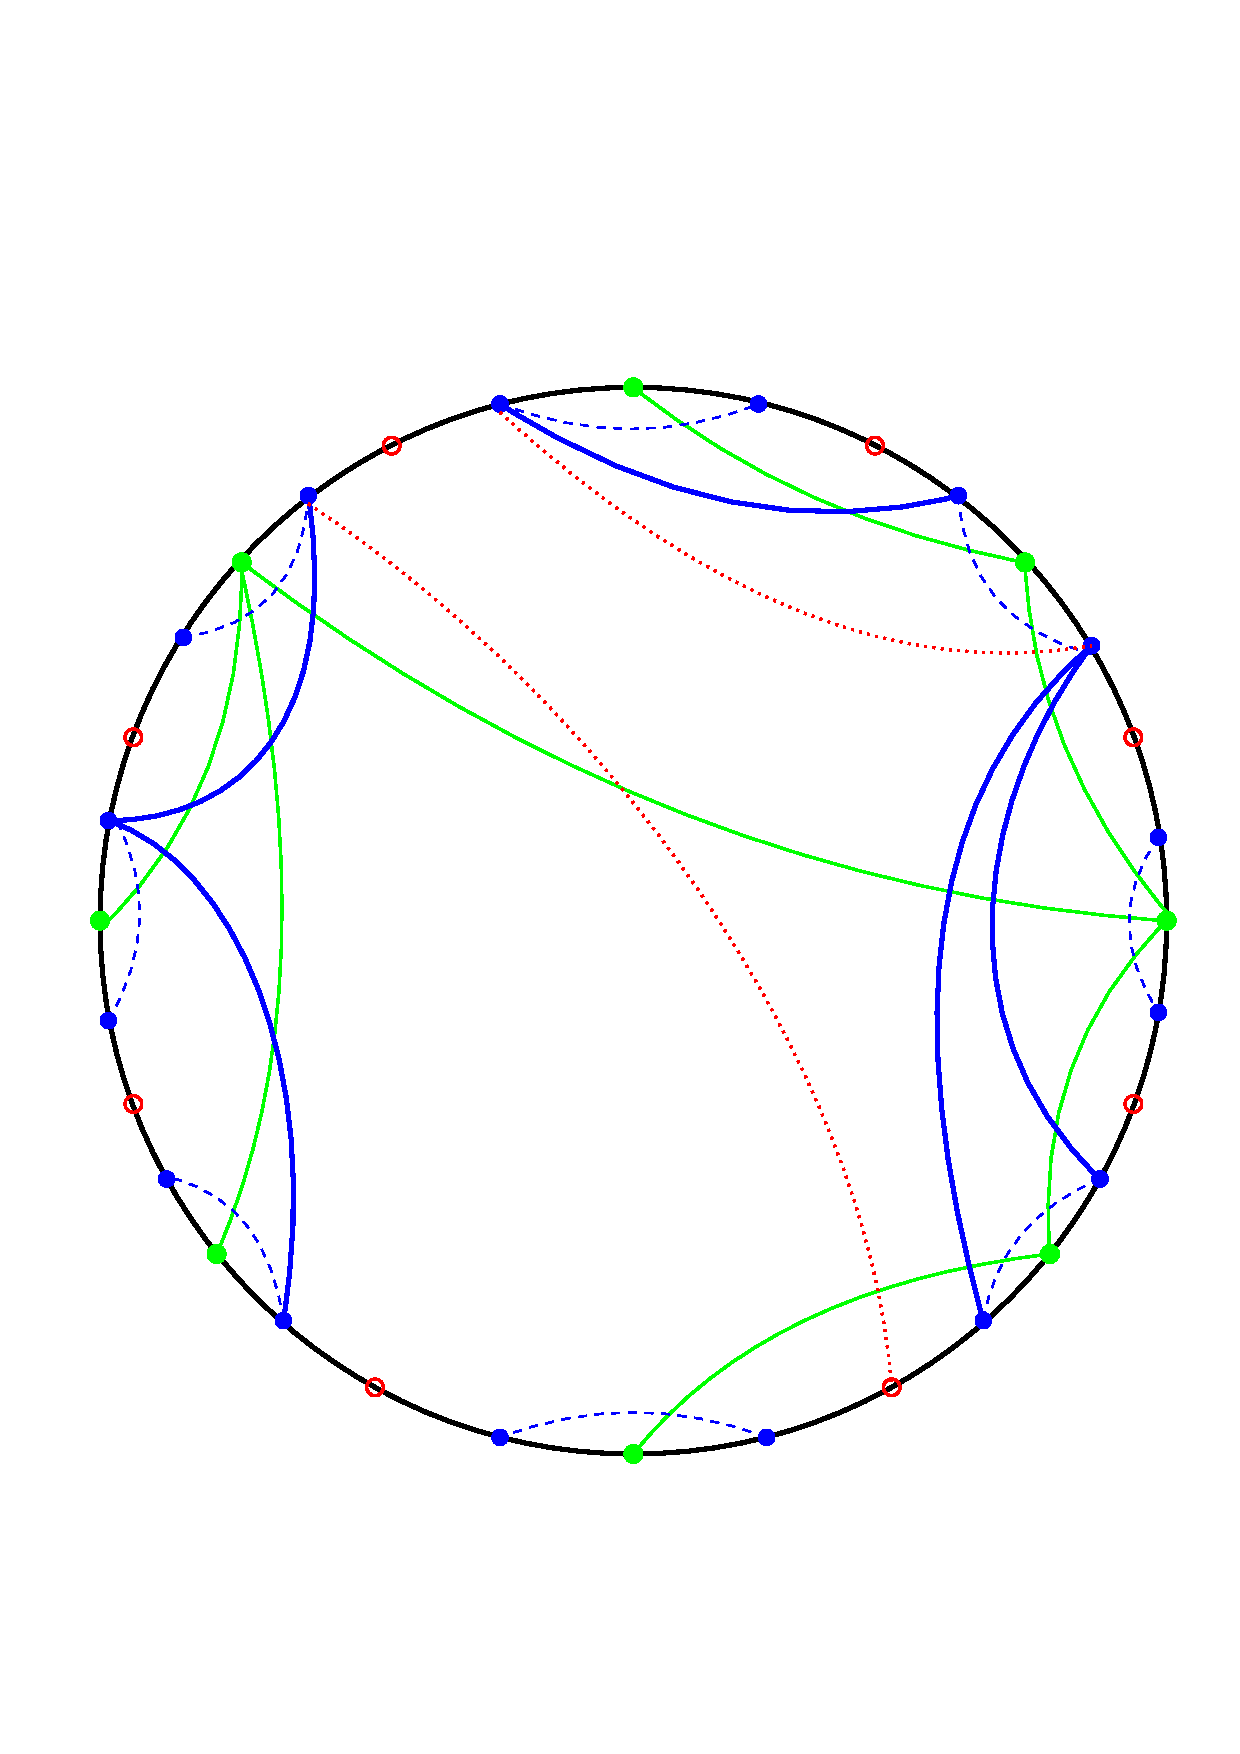
\includegraphics[scale=.17]{DissectionAccordions}

\vspace*{-3cm}
\begin{minipage}{5.7cm}
Example:

\smallskip
\begin{compactitem}
 \item A dissection (green)
 \item Some accordions (blue)
 \item Some non-accordions (red)
\end{compactitem}

\medskip
Accordions not crossing any other accordion are dotted blue.
\end{minipage}


\vspace{.3cm}
\hspace{-.25cm}
{\color{blue} \rule{10.02cm}{1pt}}
\vspace{-.35cm}

(In the language of [Manneville--Pilaud])

\smallskip

Vertices of alternating colour green-blue-red-blue.

\smallskip

{\color{blue} Dissection} $=$ collection of non-crossing green diagonals.

\smallskip

{\color{blue} Accordion} $=$ blue diagonal crossing a connected subset of the dissection (including boundary segments).


\vspace{-.1cm}
\hspace{-.25cm}
{\color{blue} \rule{10.02cm}{1pt}}
\vspace{-.35cm}

{\color{blue} (reduced) non-crossing complex} $=$ clique complex of (non-dotted) accordions of a fixed dissection for the compatibility relation of non-crossing.

\smallskip

{\color{blue} \bf Thm} [GMcC]: {\it The reduced non-crossing complex is pure and thin.}


}

%%%%%%%%%%%%%%%%%%%%%%%%%%%%%%%%%%%%%%%%%%%%%%%%%%%%%%%%%%%%%%%%%%%%%%%%%%%%%%
\headerbox{... to accordions on a Riemann surface}{name=PPP2,column=3,span=3,below=PPP1,borderColor=blue,headerColorOne=blue}{
%%%%%%%%%%%%%%%%%%%%%%%%%%%%%%%%%%%%%%%%%%%%%%%%%%%%%%%%%%%%%%%%%%%%%%%%%%%%%%

% \hspace*{6cm}
\vspace*{-.1cm}
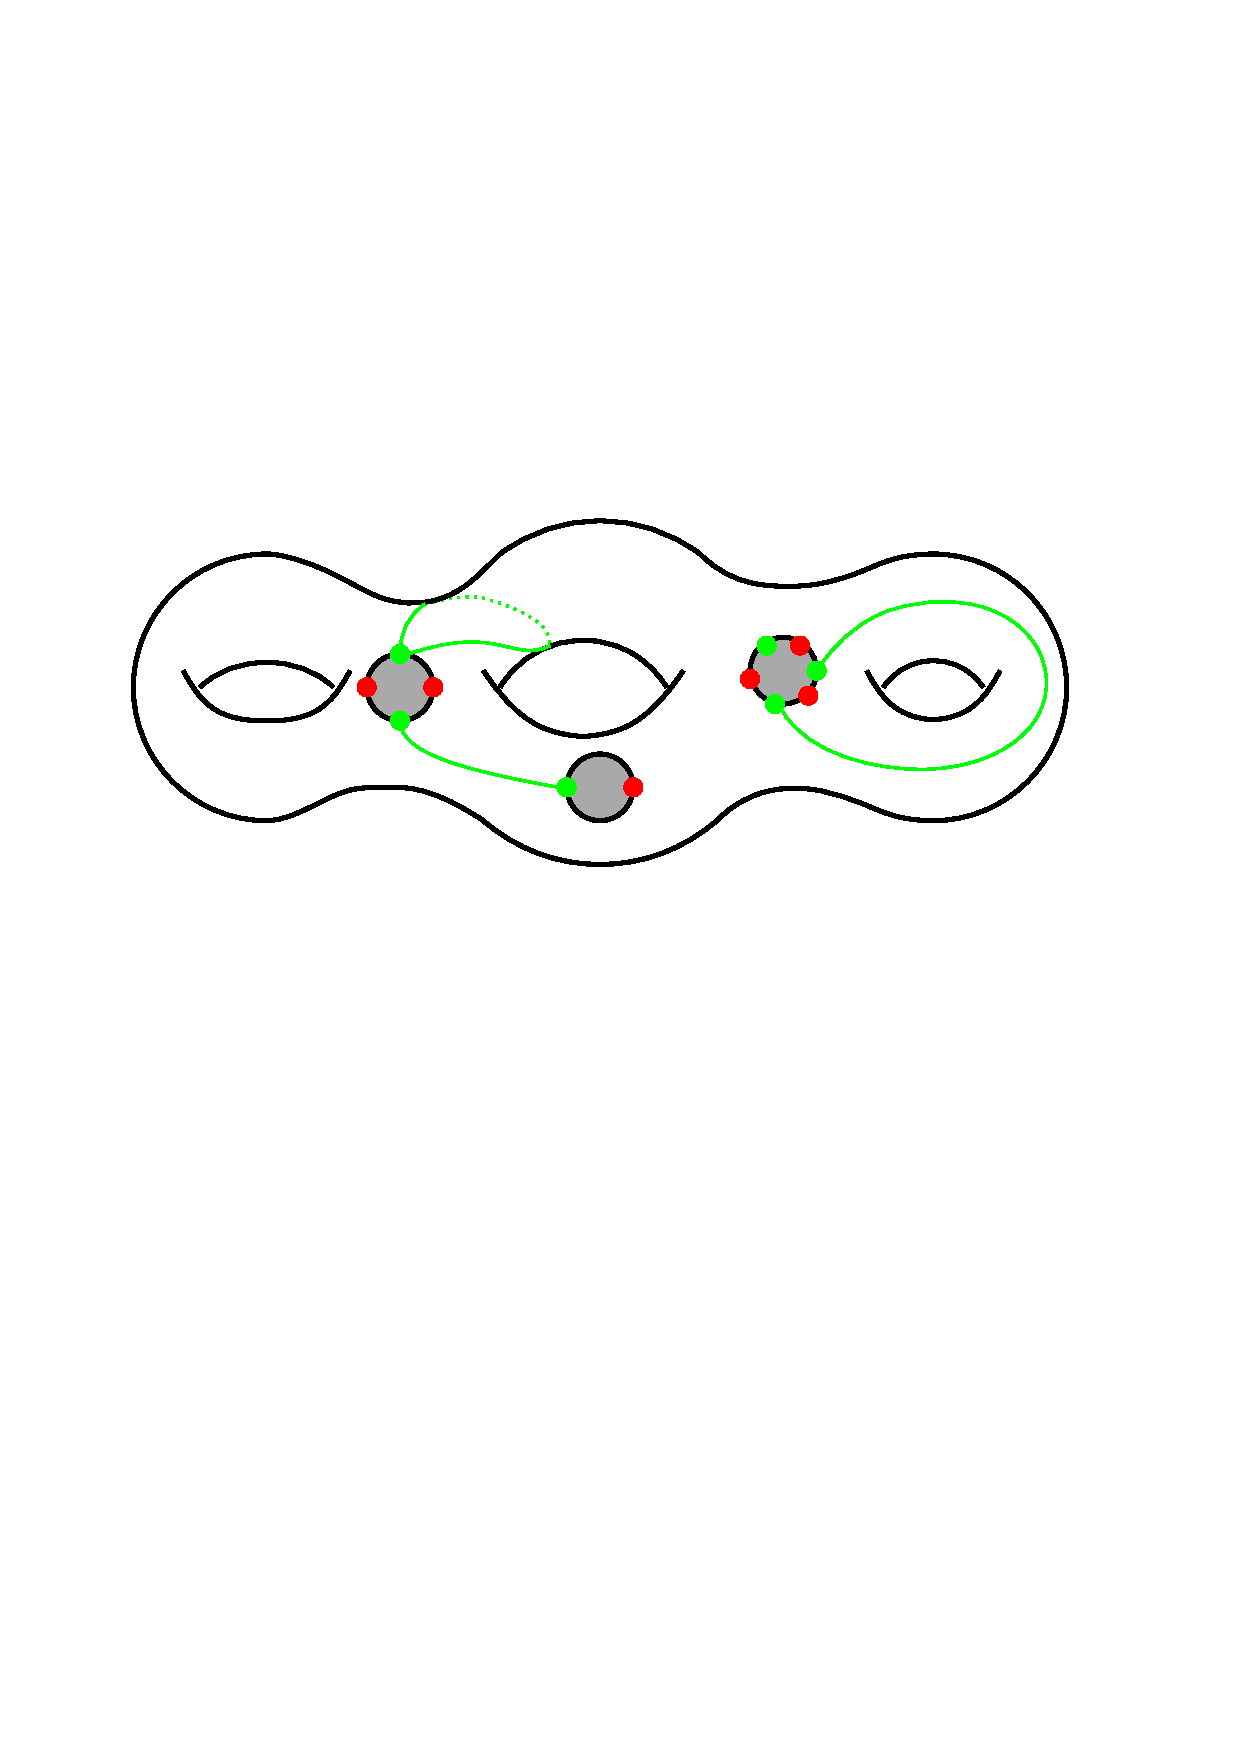
\includegraphics[scale=.35]{Surface}

\vspace*{-1.7cm}\hspace*{5.6cm}
\begin{minipage}{4cm}
{\footnotesize Some arcs on a Riemann surface with boundary and marked points.}
\end{minipage}

\vspace{.6cm}
\hspace{-.25cm}
{\color{blue} \rule{10.02cm}{1pt}}
\vspace{-.35cm}

\hspace*{6.8cm}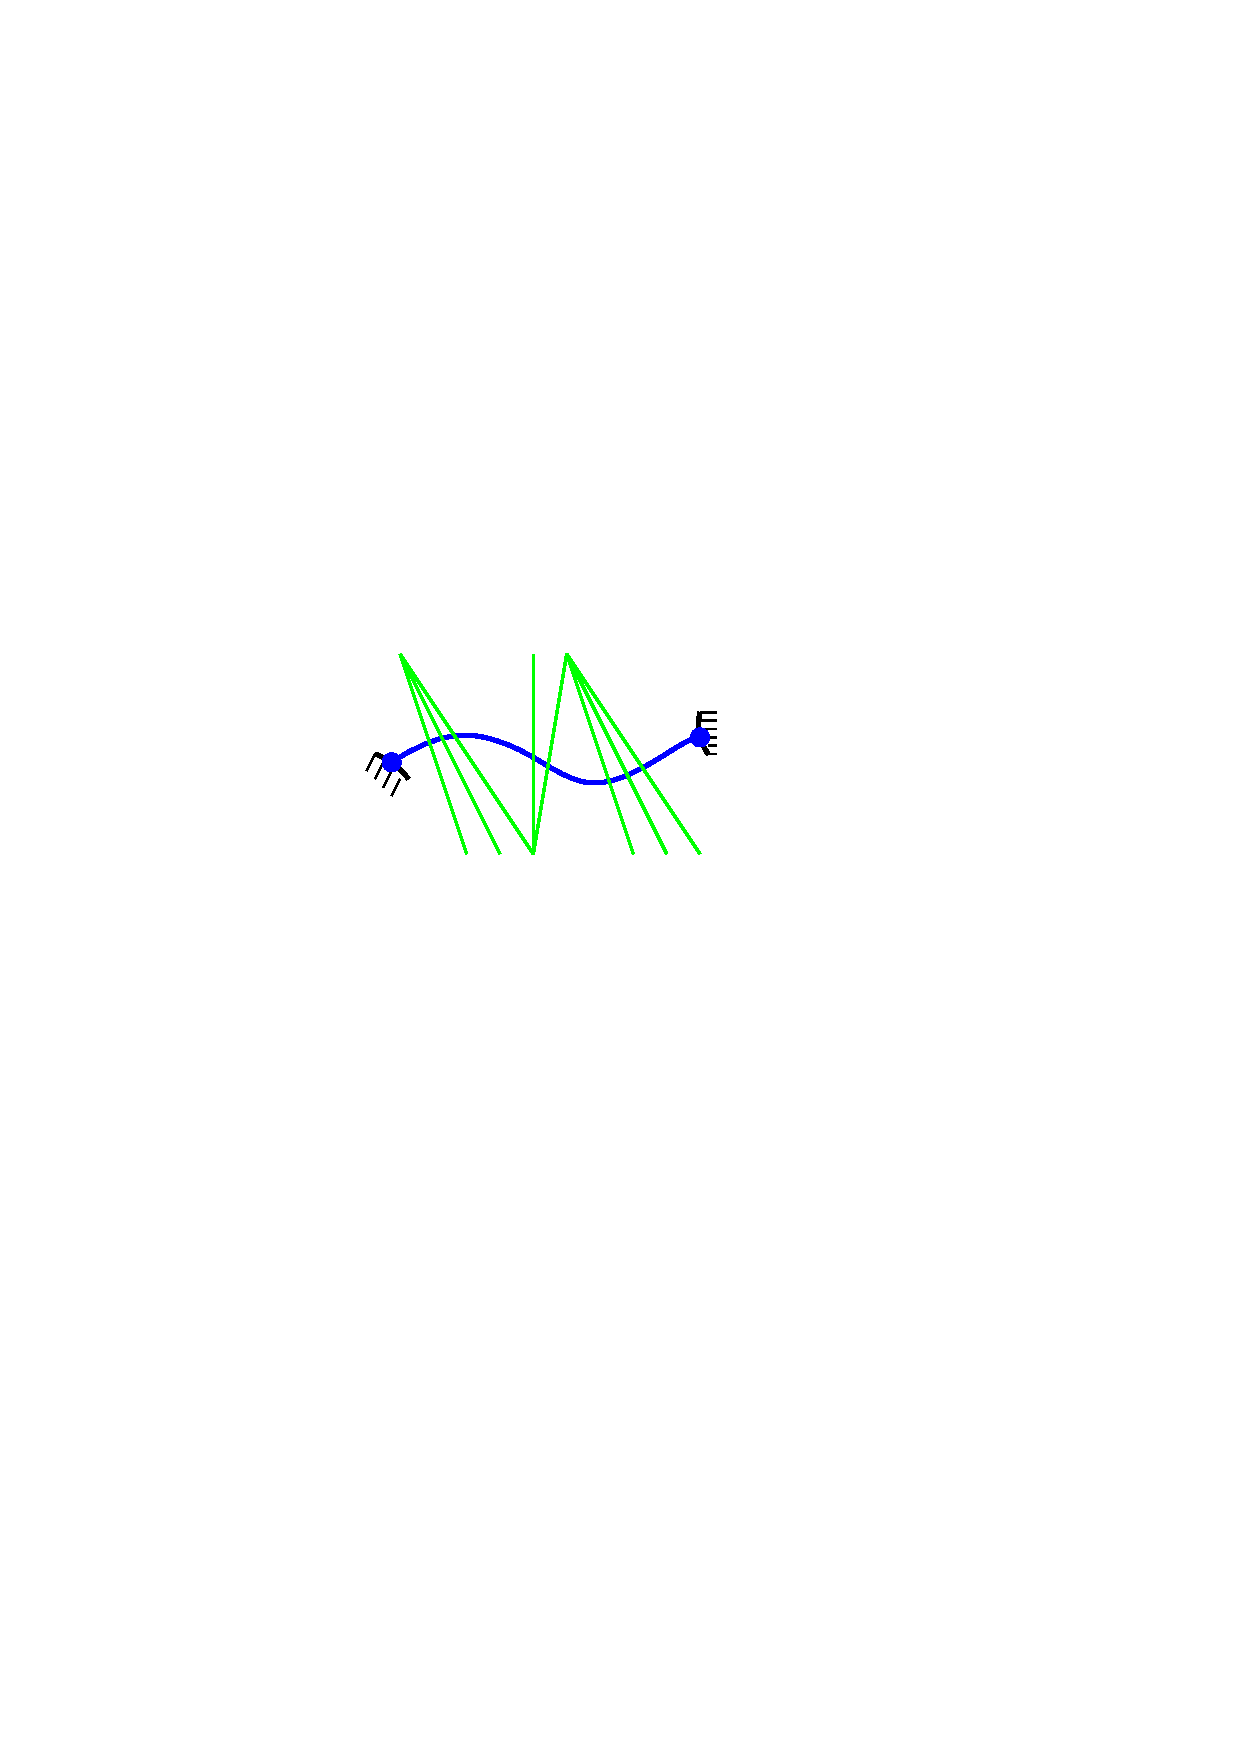
\includegraphics[scale=.5]{Accordion}

\vspace*{-1.7cm}
\begin{minipage}{6.7cm}
 Given a dualizable ($=$ every cell of the dissection contains exactly one red vertex, possibly not on the bounday) dissection of a Riemann surface, can define accordions.
\end{minipage}


\vspace{.1cm}
\hspace{-.25cm}
{\color{blue} \rule{10.02cm}{1pt}}
\vspace{-.35cm}


{\color{blue} \bf Thm} [PPP]: {\it The reduced non-crossing complex is pure and thin.}

}

%%%%%%%%%%%%%%%%%%%%%%%%%%%%%%%%%%%%%%%%%%%%%%%%%%%%%%%%%%%%%%%%%%%%%%%%%%%%%%
\headerbox{From dissections to gentle bound quivers}{name=Dissection2Gentle,column=0,span=3,below=accordions,borderColor=red,headerColorOne=red}{
%%%%%%%%%%%%%%%%%%%%%%%%%%%%%%%%%%%%%%%%%%%%%%%%%%%%%%%%%%%%%%%%%%%%%%%%%%%%%%

\hspace*{6cm}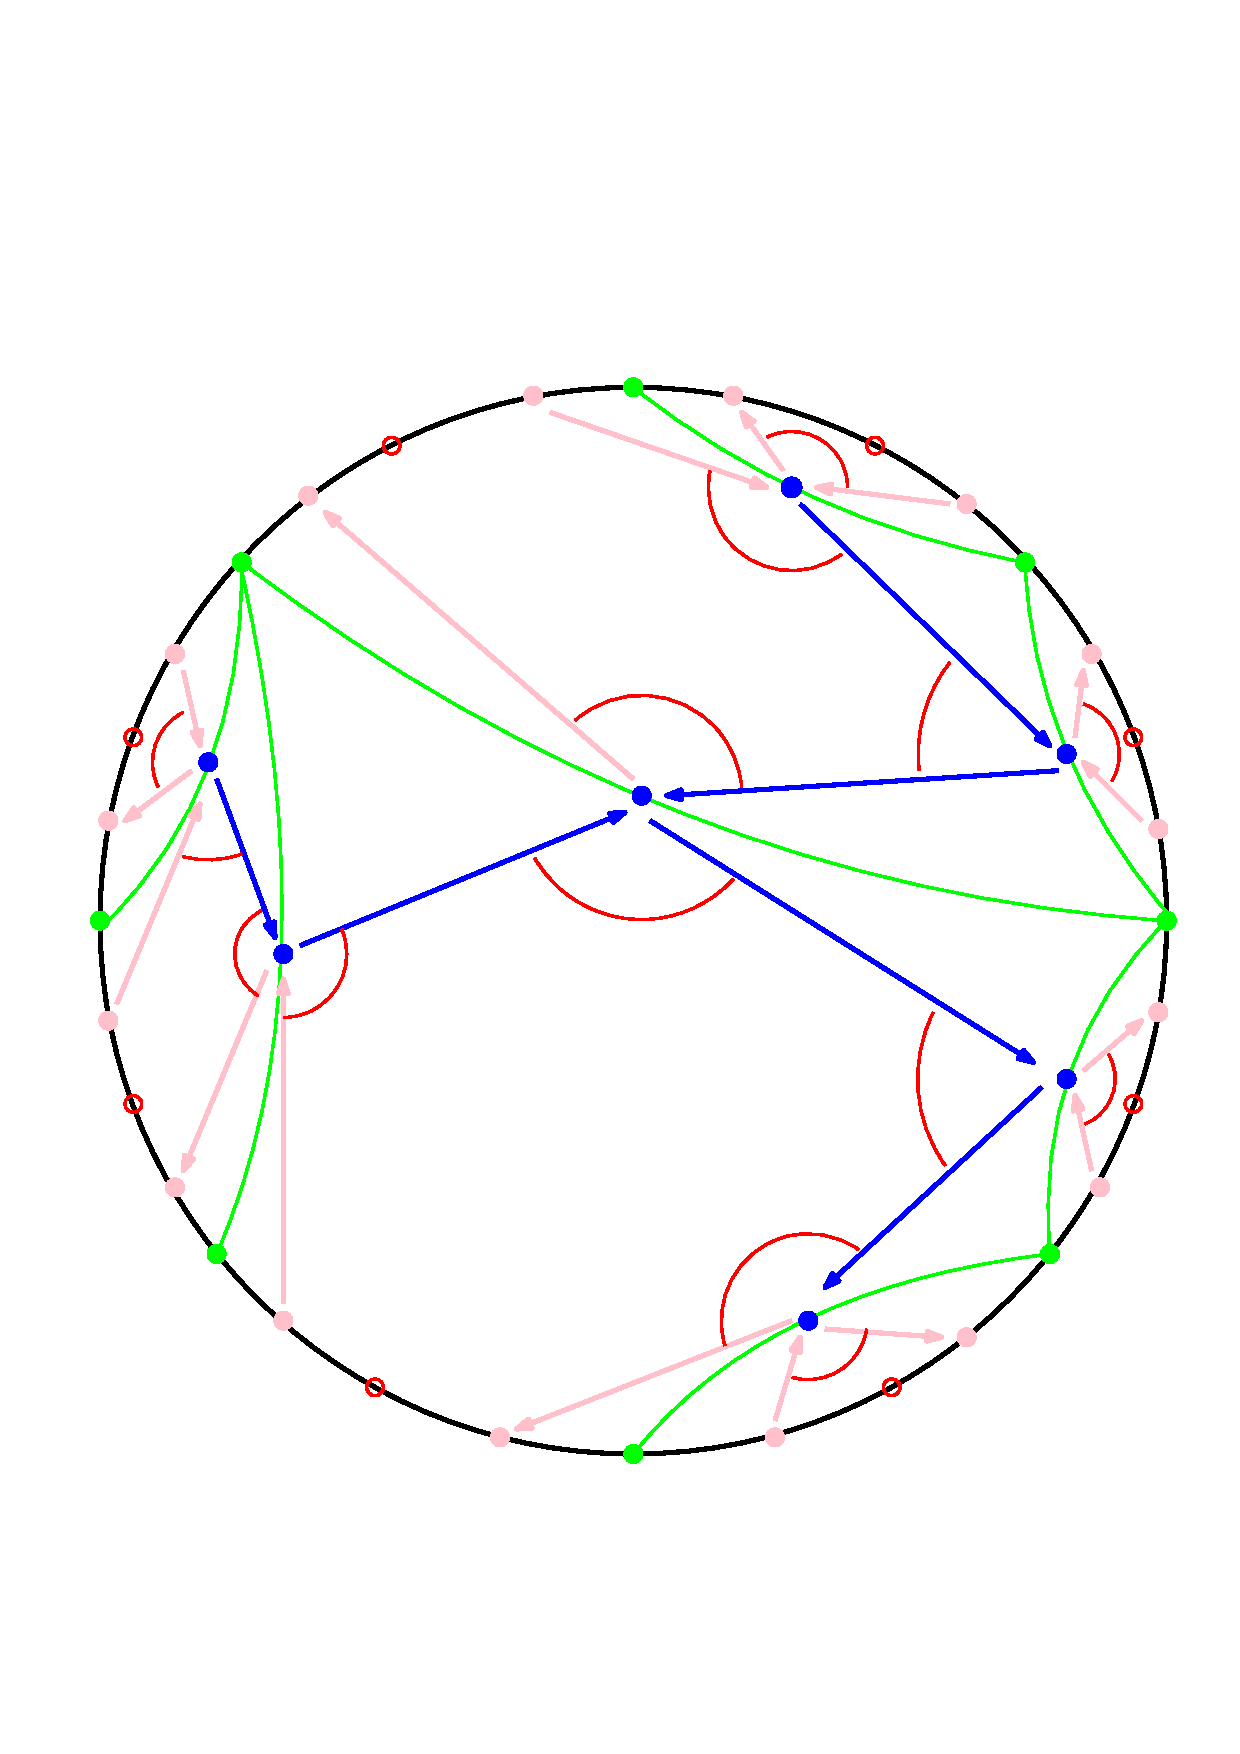
\includegraphics[scale=.2]{QuiverOfADissection}

\vspace*{-3.7cm}

\begin{minipage}{5.8cm}
Quiver of a dissection:

\smallskip

\begin{compactitem}
 \item Vertices $=$ arcs of the dissection;
 \item Arrows $=$ angles;
 \item Relations $=$ two consecutive arrows in a same cell.
\end{compactitem}

\medskip

Take boundary segments into account to obtain the blossoming.

\end{minipage}

\vspace{.55cm}
\hspace{-.25cm}
{\color{red} \rule{10.02cm}{1pt}}
\vspace{-.35cm}

{\color{red} \bf Prop:} {\it The bound quiver associated with any dualizable dissection of}
\hspace*{1cm}{\it a marked surface is gentle.}
}

%%%%%%%%%%%%%%%%%%%%%%%%%%%%%%%%%%%%%%%%%%%%%%%%%%%%%%%%%%%%%%%%%%%%%%%%%%%%%%
\headerbox{From gentle bound quivers to dissections}{name=Gentle2Dissection,column=3,span=3,below=PPP2,borderColor=red,headerColorOne=red}{
%%%%%%%%%%%%%%%%%%%%%%%%%%%%%%%%%%%%%%%%%%%%%%%%%%%%%%%%%%%%%%%%%%%%%%%%%%%%%%

\begin{center}
 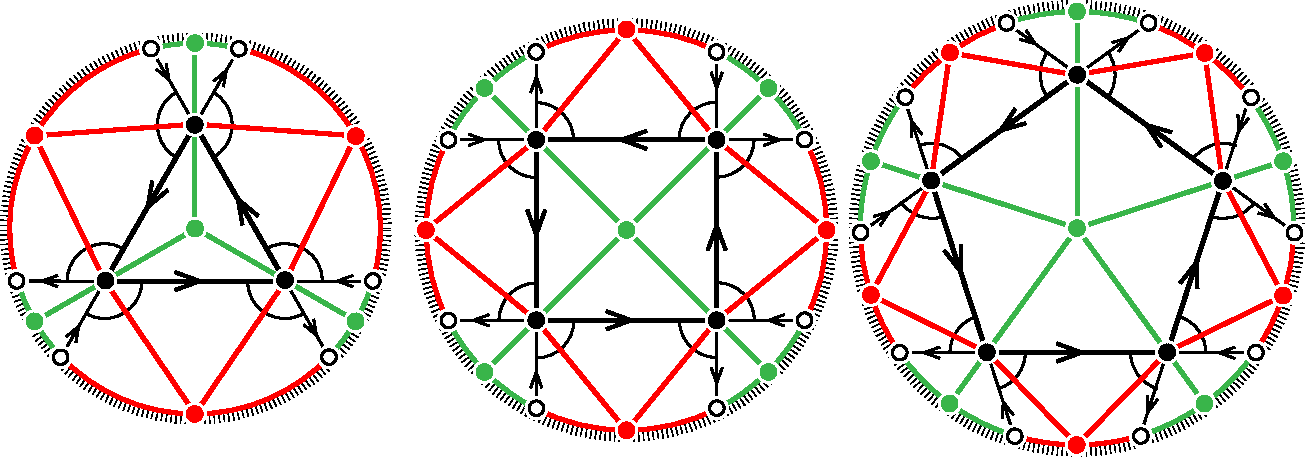
\includegraphics[scale=.3]{cyclesSurfacesBis}
 
 {\footnotesize The surface of three cyclic quivers} 
 \end{center}

\vspace{-.55cm}
\hspace{-.25cm}
{\color{red} \rule{10.02cm}{1pt}}
\vspace{-.35cm}

Given a gentle bound quiver $(Q,I)$, take its blossoming, then glue a green triangle to the left of each arrow, and a red triangle to the right of each arrow.
Glue two consecutive red (resp. green) triangles if the corresponding arrows (resp. do not) form a relation.

\vspace*{-.6cm}
\begin{center}
 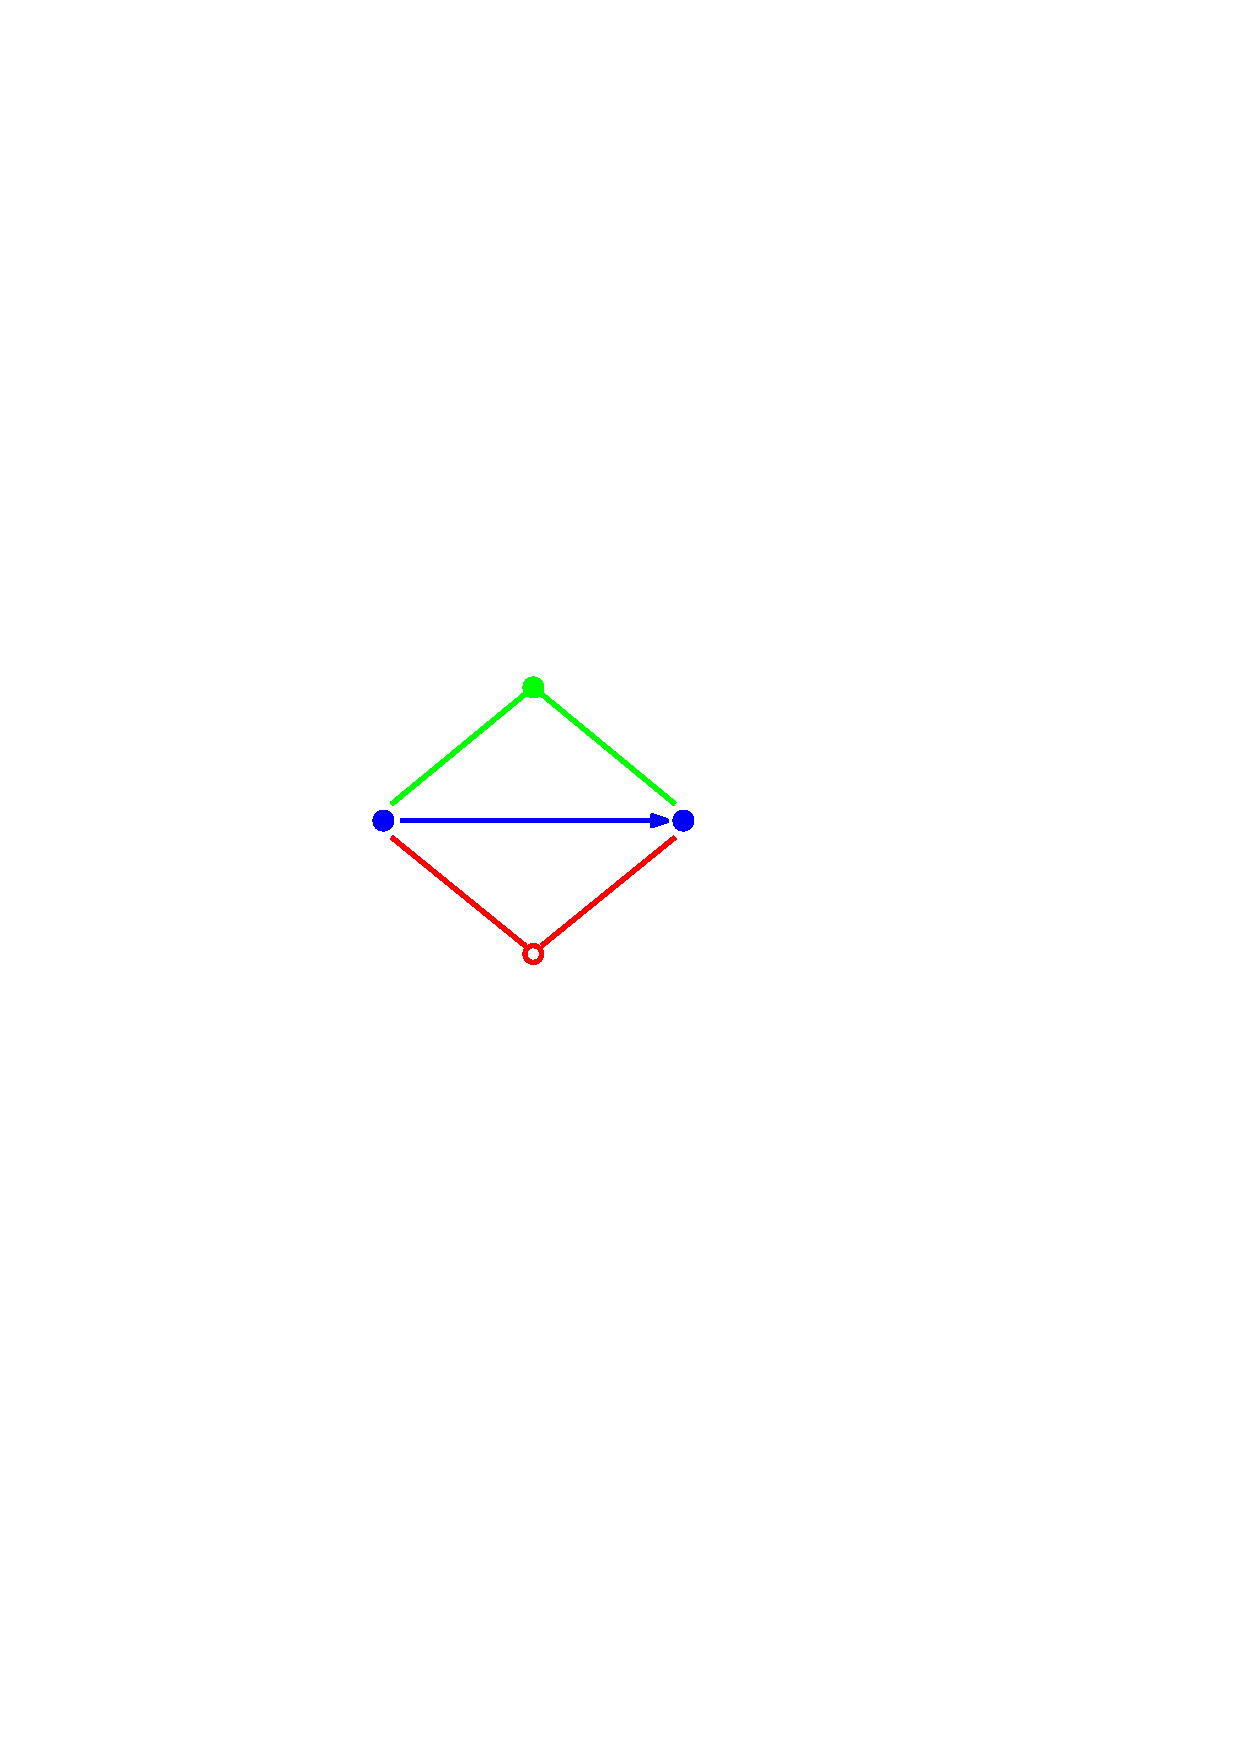
\includegraphics[scale=.3]{TrianglesArrow}\hspace*{1cm}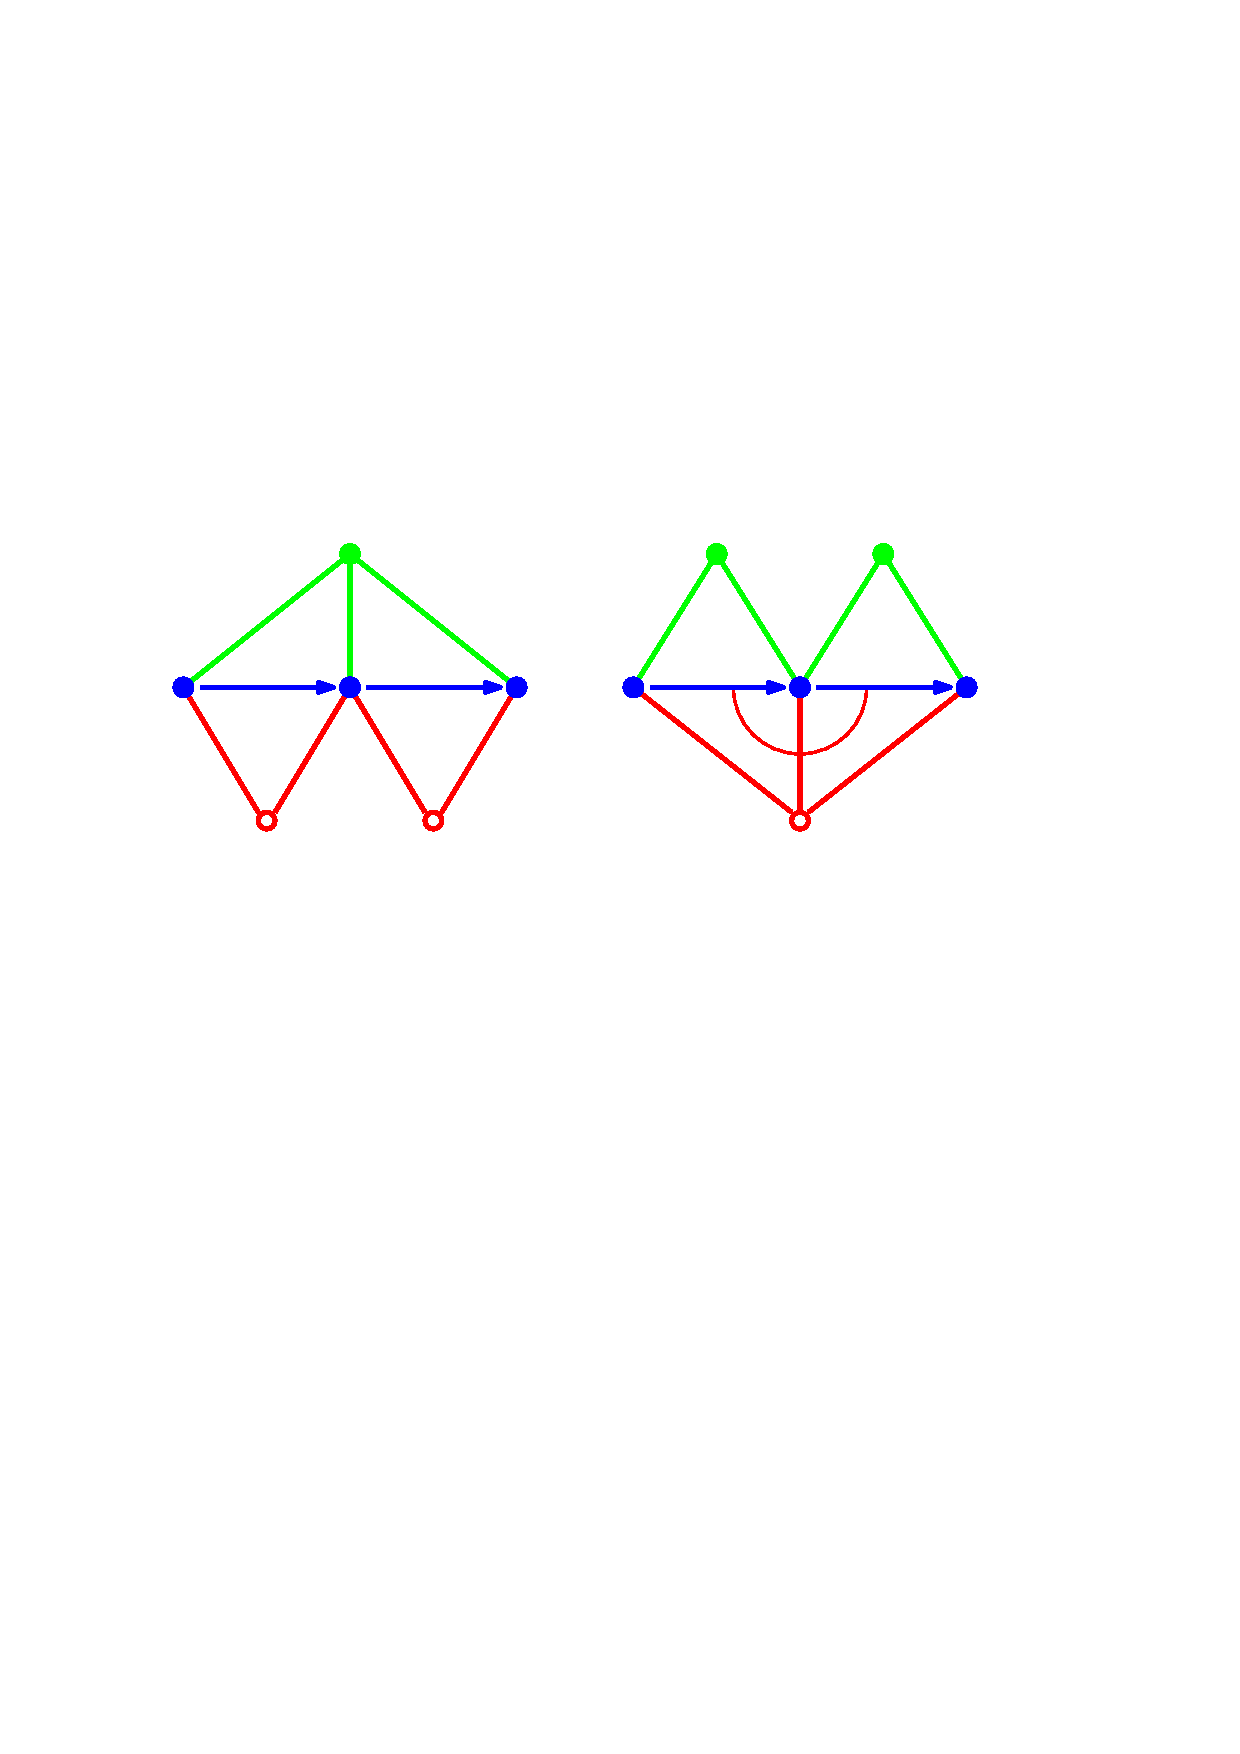
\includegraphics[scale=.35]{GlueTriangles}
\end{center}


\vspace{-.55cm}
\hspace{-.25cm}
{\color{red} \rule{10.02cm}{1pt}}
\vspace{-.35cm}

{\color{red} \bf Prop:} {\it The construction above yields a marked surface endowed with}
\hspace*{1cm}{\it a pair of dual dissections; given by green arcs / red arcs.}

}



%%%%%%%%%%%%%%%%%%%%%%%%%%%%%%%%%%%%%%%%%%%%%%%%%%%%%%%%%%%%%%%%%%%%%%%%%%%%%%
\headerbox{Main Results [PPP]}{name=polytopes,column=0,span=3,below=Dissection2Gentle,borderColor=red,headerColorOne=red}{
%%%%%%%%%%%%%%%%%%%%%%%%%%%%%%%%%%%%%%%%%%%%%%%%%%%%%%%%%%%%%%%%%%%%%%%%%%%%%%

{\color{red} \bf Thm:} {\it gentle bound quivers $\longleftrightarrow$ marked oriented surfaces with}
\hspace*{1.05cm}{\it boundary endowed with a pair of dual dissections.}

\vspace{-.15cm}
\hspace{-.25cm}
{\color{red} \rule{10.02cm}{1pt}}
\vspace{-.35cm}

{\color{red} \bf Thm:} {\it
Walks on $(Q,I)$ $\longleftrightarrow$ accordions on the associated surface $S$

\hspace*{2.25cm}kissing $\longleftrightarrow$ crossing

non-kissing complex of $(Q,I)$ $\cong$ non-crossing complex of $S$.
}
}


%%%%%%%%%%%%%%%%%%%%%%%%%%%%%%%%%%%%%%%%%%%%%%%%%%%%%%%%%%%%%%%%%%%%%%%%%%%%%%
\headerbox{Relation with representation theory}{name=polytopes,column=3,span=3,below=Gentle2Dissection,borderColor=black,headerColorOne=black}{
%%%%%%%%%%%%%%%%%%%%%%%%%%%%%%%%%%%%%%%%%%%%%%%%%%%%%%%%%%%%%%%%%%%%%%%%%%%%%%

arXiv:1707.07574 -- NKC and tau-tilting for gentle algebras

arXiv:1807.04730 -- NKC and NCC for locally gentle algebras

}

% \includegraphics[width=1.03\textwidth]{PermBrickZono2}
% 
% \begin{tabular}{c@{\quad}c@{\qquad}c}
% {\color{blue} $\Perm[]$} & {\color{red} $\Brick$} & {\color{green} $\Zono$} \\
% $\conv\set{\b{x}(\tau)}{\tau \in \fS_n}$ & $\conv\set{\b{b}(\twist)}{\twist \text{ $(k,n)$-twist}}$ & $\sum_{|i-j| < k} \; [\b{e}_i, \b{e}_j]$ \\
% $\b{x}(\tau)_i = \tau(i)$ & $\b{b}(\twist)_i =$ nbr bricks below pipe~$i$
% \end{tabular}
% 
% }
% 
% %%%%%%%%%%%%%%%%%%%%%%%%%%%%%%%%%%%%%%%%%%%%%%%%%%%%%%%%%%%%%%%%%%%%%%%%%%%%%%
% \headerbox{Matriochka polytopes}{name=matriochka,column=4,span=2,below=twists,borderColor=green,headerColorOne=green}{
% %%%%%%%%%%%%%%%%%%%%%%%%%%%%%%%%%%%%%%%%%%%%%%%%%%%%%%%%%%%%%%%%%%%%%%%%%%%%%%
% 
% \centerline{\footnotesize {\color{blue} $\Perm[]$} $\;\subset\;$ {\color{red} $\Brick$} $\;\subset\;$ {\color{green} $\Zono$}}
% \vspace{.1cm}
% \centerline{\includegraphics[scale=.3]{PermBrickZonoInclusionsBis}}
% 
% \vspace{-2.1cm}\hspace{.3cm}{\footnotesize $k=1$}
% 
% \vspace{1.1cm}\hspace{5.3cm}{\footnotesize $k=2$}
% 
% \vspace{-.1cm}
% \hspace{-.25cm}
% {\color{green} \rule{6.6cm}{1pt}}
% \vspace{-.47cm}
% 
% \centerline{\footnotesize ${\color{red} \Brick[1]} \! \subset \! {\color{orange} \Brick[2]} \! \subset \! {\color{green} \Brick[3]} \! \subset \! \cdots \! \subset \! {\color{blue} \Perm}$}
% \vspace{.1cm}
% \centerline{\includegraphics[scale=.3]{geometricInclusions}}
% \vspace{-.1cm}
% \centerline{\footnotesize ${\color{red} \Zono[1]} \! \subset \! {\color{orange} \Zono[2]} \! \subset \! {\color{green} \Zono[3]} \! \subset \! \cdots \! \subset \! {\color{blue} \Perm}$}
% }
% 
% %%%%%%%%%%%%%%%%%%%%%%%%%%%%%%%%%%%%%%%%%%%%%%%%%%%%%%%%%%%%%%%%%%%%%%%%%%%%%%
% \headerbox{Hopf algebras}{name=twistAlgebra,column=0,span=3,below=polytopes,borderColor=blue,headerColorOne=blue}{
% %%%%%%%%%%%%%%%%%%%%%%%%%%%%%%%%%%%%%%%%%%%%%%%%%%%%%%%%%%%%%%%%%%%%%%%%%%%%%%
% 
% {\color{blue} Malvenuto-Reutenauer Hopf algebra} $=$ basis~$(\F_\tau)_{\tau \in \fS}$ and
% \[
% \F_\tau \product \F_{\tau'} = \sum_{\sigma \in \tau \shiftedShuffle \tau'} \F_\sigma
% \qquad\text{and}\qquad
% \coproduct \F_\sigma = \sum_{\sigma \in \tau \convolution \tau'} \F_\tau \otimes \F_{\tau'}
% \]
% 
% {\scriptsize
% $\!\!\begin{array}[t]{@{}r@{\,=\,}l}
% {\color{red} 1}{\color{red} 2} \shiftedShuffle {\color{blue} 23}{\color{blue} 1} & \{ {\color{red} 1}{\color{red} 2}{\color{blue} 45}{\color{blue} 3}, {\color{red} 1}{\color{blue} 4}{\color{red} 2}{\color{blue} 5}{\color{blue} 3}, {\color{red} 1}{\color{blue} 45}{\color{red} 2}{\color{blue} 3}, {\color{red} 1}{\color{blue} 45}{\color{blue} 3}{\color{red} 2}, {\color{blue} 4}{\color{red} 1}{\color{red} 2}{\color{blue} 5}{\color{blue} 3}, {\color{blue} 4}{\color{red} 1}{\color{blue} 5}{\color{red} 2}{\color{blue} 3}, {\color{blue} 4}{\color{red} 1}{\color{blue} 5}{\color{blue} 3}{\color{red} 2}, {\color{blue} 45}{\color{red} 1}{\color{red} 2}{\color{blue} 3}, {\color{blue} 45}{\color{red} 1}{\color{blue} 3}{\color{red} 2}, {\color{blue} 45}{\color{blue} 3}{\color{red} 1}{\color{red} 2} \} \\
% {\color{red} 1}{\color{red} 2} \convolution {\color{blue} 23}{\color{blue} 1} & \{ {\color{red} 1}{\color{red} 2}{\color{blue} 45}{\color{blue} 3}, {\color{red} 1}{\color{red} 3}{\color{blue} 45}{\color{blue} 2}, {\color{red} 1}{\color{red} 4}{\color{blue} 35}{\color{blue} 2}, {\color{red} 1}{\color{red} 5}{\color{blue} 34}{\color{blue} 2}, {\color{red} 2}{\color{red} 3}{\color{blue} 45}{\color{blue} 1}, {\color{red} 2}{\color{red} 4}{\color{blue} 35}{\color{blue} 1}, {\color{red} 2}{\color{red} 5}{\color{blue} 34}{\color{blue} 1}, {\color{red} 3}{\color{red} 4}{\color{blue} 25}{\color{blue} 1}, {\color{red} 3}{\color{red} 5}{\color{blue} 24}{\color{blue} 1}, {\color{red} 4}{\color{red} 5}{\color{blue} 23}{\color{blue} 1} \}
% \end{array}$
% }
% 
% \vspace{-.3cm}
% \hspace{-.25cm}
% {\color{blue} \rule{10.02cm}{1pt}}
% 
% {\color{blue} $k$-twist algebra} $=$ \uline{subalgebra} of MR algebra generated by \\
% $\PTwist_{\twist} \eqdef \!\! \sum\limits_{\surjectionPermBrick(\tau) = \twist} \!\! \F_\tau = \!\! \sum\limits_{\tau \in \linearExtensions(\twist\contact)} \!\! \F_\tau$ for all acyclic~$k$-twists~$\twist$
% %\qquad\qquad\qquad $\PTwist\raisebox{.1cm}{$_{\hspace{-.2cm}\includegraphics[scale=.5]{exmTwist2}}$} = \!\!\!\! \begin{array}[t]{c} \phantom{+} \; \F_{31542} \\ + \; \F_{35142} \end{array}$
% 
% \smallskip
% Exm: $k = 1$ $\;\Longrightarrow\;$ Loday-Ronco Hopf algebra on binary trees
% 
% \vspace{-.15cm}
% \hspace{-.25cm}
% {\color{blue} \rule{10.02cm}{1pt}}
% 
% {\color{blue} $k$-recoil algebra} $=$ \uline{subalgebra} of MR algebra generated by \\
% $\X_{\orientation} \eqdef \!\!\!\!\! \sum\limits_{\surjectionPermZono(\tau) = \orientation} \!\!\!\!\! \F_\tau$ for all acyclic orientations~$\orientation$ of~$\Gkn$ for $n \in \N$
% 
% \smallskip
% Exm: $k = 1$ $\;\Longrightarrow\;$ Solomon descent algebra
% 
% \vspace{-.15cm}
% \hspace{-.25cm}
% {\color{blue} \rule{10.02cm}{1pt}}
% 
% Matriochkas:
% \begin{tabular}[t]{@{}l} 
% $\bullet$ $k$-recoil alg. $\hookrightarrow$ $k$-twist alg. $\hookrightarrow$ MR alg. \\
% $\bullet$ if $\ell< k$, \, $\ell$-rec $\hookrightarrow$ $k$-rec \, and \, $\ell$-twist $\hookrightarrow$ $k$-twist
% \end{tabular}
% 
% \vspace{-.1cm}
% }
% 
% %%%%%%%%%%%%%%%%%%%%%%%%%%%%%%%%%%%%%%%%%%%%%%%%%%%%%%%%%%%%%%%%%%%%%%%%%%%%%%
% \headerbox{Products}{name=product,column=3,span=3,below=polytopes,borderColor=blue,headerColorOne=blue}{
% %%%%%%%%%%%%%%%%%%%%%%%%%%%%%%%%%%%%%%%%%%%%%%%%%%%%%%%%%%%%%%%%%%%%%%%%%%%%%%
% 
% {\scriptsize
%     \centerline{$
%     \begin{array}{@{}c@{\;=\;}c@{\;+\;}c@{\;+ \cdots +\;}c}%c@{+}c@{+}c@{+}c@{}}
%     \PTwist\raisebox{.1cm}{$_{\hspace{-.2cm}\includegraphics[scale=.65]{exmProduct/exmProduct1}}$} \product \PTwist\raisebox{.1cm}{$_{\hspace{-.2cm}\includegraphics[scale=.65]{exmProduct/exmProduct2}}$} & 
%     \multicolumn{3}{@{}l}{(\F_{\color{red} 1423} + \F_{\color{red} 4123}) \product \F_{\color{blue} 21}}
%     \\[-1.1cm]
%     & \begin{bmatrix} \phantom{+ \, } \F_{{\color{red} 1423}{\color{blue} 65}} \\ + \, \F_{{\color{red} 4123}{\color{blue} 65}} \end{bmatrix}
%     & \begin{bmatrix} \phantom{+ \, } \F_{{\color{red} 142}{\color{blue} 6}{\color{red} 3}{\color{blue} 5}} \\ + \, \F_{{\color{red} 14}{\color{blue} 6}{\color{red} 23}{\color{blue} 5}} \\ + \, \F_{{\color{red} 412}{\color{blue} 6}{\color{red} 3}{\color{blue} 5}} \\ + \, \F_{{\color{red} 41}{\color{blue} 6}{\color{red} 23}{\color{blue} 5}} \\ + \, \F_{{\color{red} 4}{\color{blue} 6}{\color{red} 123}{\color{blue} 5}} \end{bmatrix}
% %    & \begin{bmatrix} \phantom{+ \, } \F_{{\color{red} 1}{\color{blue} 6}{\color{red} 423}{\color{blue} 5}} \\ + \, \F_{{\color{blue} 6}{\color{red} 1423}{\color{blue} 5}} \\ + \, \F_{{\color{blue} 6}{\color{red} 4123}{\color{blue} 5}} \end{bmatrix}
% %    & \begin{bmatrix} \phantom{+ \, } \F_{{\color{red} 142}{\color{blue} 65}{\color{red} 3}} \\ + \, \F_{{\color{red} 14}{\color{blue} 6}{\color{red} 2}{\color{blue} 5}{\color{red} 3}} \\ + \, \F_{{\color{red} 412}{\color{blue} 65}{\color{red} 3}} \\ + \, \F_{{\color{red} 41}{\color{blue} 6}{\color{red} 2}{\color{blue} 5}{\color{red} 3}} \\ + \, \F_{{\color{red} 4}{\color{blue} 6}{\color{red} 12}{\color{blue} 5}{\color{red} 3}} \end{bmatrix}
% %    & \begin{bmatrix} \phantom{+ \, } \F_{{\color{red} 1}{\color{blue} 6}{\color{red} 42}{\color{blue} 5}{\color{red} 3}} \\ + \, \F_{{\color{blue} 6}{\color{red} 142}{\color{blue} 5}{\color{red} 3}} \\ + \, \F_{{\color{blue} 6}{\color{red} 412}{\color{blue} 5}{\color{red} 3}} \end{bmatrix}
% %    & \begin{bmatrix} \phantom{+ \, } \F_{{\color{red} 14}{\color{blue} 65}{\color{red} 23}} \\ + \, \F_{{\color{red} 41}{\color{blue} 65}{\color{red} 23}} \\ + \, \F_{{\color{red} 4}{\color{blue} 6}{\color{red} 1}{\color{blue} 5}{\color{red} 23}} \\ + \, \F_{{\color{red} 4}{\color{blue} 65}{\color{red} 123}} \end{bmatrix}
% %    & \begin{bmatrix} \phantom{+ \, } \F_{{\color{red} 1}{\color{blue} 6}{\color{red} 4}{\color{blue} 5}{\color{red} 23}} \\ + \, \F_{{\color{blue} 6}{\color{red} 14}{\color{blue} 5}{\color{red} 23}} \\ + \, \F_{{\color{blue} 6}{\color{red} 41}{\color{blue} 5}{\color{red} 23}} \\ + \, \F_{{\color{blue} 6}{\color{red} 4}{\color{blue} 5}{\color{red} 123}} \end{bmatrix}
%     & \begin{bmatrix} \phantom{+ \, } \F_{{\color{red} 1}{\color{blue} 65}{\color{red} 423}} \\ + \, \F_{{\color{blue} 6}{\color{red} 1}{\color{blue} 5}{\color{red} 423}} \\ + \, \F_{{\color{blue} 65}{\color{red} 1423}} \\ + \, \F_{{\color{blue} 65}{\color{red} 4123}} \end{bmatrix}
%     \\[.5cm]
%     & \PTwist\raisebox{.1cm}{$_{\hspace{-.2cm}\includegraphics[scale=.65]{exmProduct/exmProduct3}}$}
%     & \PTwist\raisebox{.1cm}{$_{\hspace{-.2cm}\includegraphics[scale=.65]{exmProduct/exmProduct4}}$}
% %    & \PTwist\raisebox{.1cm}{$_{\hspace{-.2cm}\includegraphics[scale=.65]{exmProduct/exmProduct5}}$}
% %    & \PTwist\raisebox{.1cm}{$_{\hspace{-.2cm}\includegraphics[scale=.65]{exmProduct/exmProduct6}}$}
% %    & \PTwist\raisebox{.1cm}{$_{\hspace{-.2cm}\includegraphics[scale=.65]{exmProduct/exmProduct7}}$}
% %    & \PTwist\raisebox{.1cm}{$_{\hspace{-.2cm}\includegraphics[scale=.65]{exmProduct/exmProduct8}}$}
% %    & \PTwist\raisebox{.1cm}{$_{\hspace{-.2cm}\includegraphics[scale=.65]{exmProduct/exmProduct9}}$}
%     & \PTwist\raisebox{.1cm}{$_{\hspace{-.2cm}\includegraphics[scale=.65]{exmProduct/exmProduct10}}$}
%     \end{array}
%     $}
% }
% \vspace{-.15cm}
% {\footnotesize \hspace{3.3cm} $\underprod{\twist}{\twist'}$ \hspace{4cm} $\overprod{\twist}{\twist'}$}
% 
% \medskip
% {\color{blue} \textsc{prop.}} $\PTwist_{\twist} \product \PTwist_{\twist'}  = \sum_{\twist[S]} \PTwist_{\twist[S]}$ where~$\twist[S]$ runs over the interval \\ between~$\underprod{\twist}{\twist'}$ and~$\overprod{\twist}{\twist'}$ in the $(k,n+n')$-twist lattice
% 
% }
% 
% %%%%%%%%%%%%%%%%%%%%%%%%%%%%%%%%%%%%%%%%%%%%%%%%%%%%%%%%%%%%%%%%%%%%%%%%%%%%%%
% \headerbox{Further topics...\qquad\qquad\quad\;{\normalsize \href{http://arxiv.org/abs/1505.07665}{\texttt{arXiv:1505.07665}}}}{name=more,column=3,span=3,below=product,borderColor=black,headerColorOne=black}{
% %%%%%%%%%%%%%%%%%%%%%%%%%%%%%%%%%%%%%%%%%%%%%%%%%%%%%%%%%%%%%%%%%%%%%%%%%%%%%%
% 
% Multiplicative bases, $k$-twistiform algebras, \dots \\
% Cambrian, tuples, Schr\"oder extensions
% 
% }
% 
% %%%%%%%%%%%%%%%%%%%%%%%%%%%%%%%%%%%%%%%%%%%%%%%%%%%%%%%%%%%%%%%%%%%%%%%%%%%%%%%
% %\headerbox{Bijection to (multi)triangulations}{name=bijection,column=3,span=3,row=0,borderColor=red,headerColorOne=red}{
% %%%%%%%%%%%%%%%%%%%%%%%%%%%%%%%%%%%%%%%%%%%%%%%%%%%%%%%%%%%%%%%%%%%%%%%%%%%%%%%
% %
% %\vspace{-.15cm}
% %\centerline{\includegraphics[scale=.95]{dualiteTriangulation}}
% %\begin{tabular}{@{}c@{$\;\;\longleftrightarrow\;\;$}c@{$\;\;\longleftrightarrow\;\;$}c}
% %$(1,n)$-twist & binary tree & triangulation $(n+2)$-gon \\
% %pipe & node & triangle \\
% %contact & arc & diagonal
% %\end{tabular}
% %\vspace{-.2cm}
% %
% %}
% 
% %%%%%%%%%%%%%%%%%%%%%%%%%%%%%%%%%%%%%%%%%%%%%%%%%%%%%%%%%%%%%%%%%%%%%%%%%%%%%%%
% %\headerbox{$k$-twist insertion algorithm}{name=insertion,column=0,span=6,below=twists,borderColor=red,headerColorOne=red}{
% %%%%%%%%%%%%%%%%%%%%%%%%%%%%%%%%%%%%%%%%%%%%%%%%%%%%%%%%%%%%%%%%%%%%%%%%%%%%%%%
% %
% %\textbf{Input}: permutation $\tau \in \fS_n$ \hspace{.5cm}
% %\textbf{Algo}: Insert pipes from right to left {\color{red} as northwest as possible} \hspace{.5cm}
% %\textbf{Output}: acyclic $(k,n)$-twist~$\surjectionPermBrick(\tau)$ \\
% %%
% %\centerline{\includegraphics[width=\textwidth]{insertion}}
% %
% %\vspace{-.8cm}\hspace{18cm}
% %$\surjectionPermBrick[2](31542)$
% %
% %\vspace{.3cm}
% %\begin{tabular}[t]{@{}l}
% %$\surjectionPermBrick$ $=$ {\color{red} surjection} permutations of~$[n]$ $\longrightarrow$ acyclic $(k,n)$-twists \quad
% %fiber of a $(k,n)$-twist~$\twist$ $=$ {\color{red} linear extensions} of its contact graph~$\twist\contact$
% %\end{tabular}
% %
% %}
% 
% %%%%%%%%%%%%%%%%%%%%%%%%%%%%%%%%%%%%%%%%%%%%%%%%%%%%%%%%%%%%%%%%%%%%%%%%%%%%%%%
% %\headerbox{Permutahedra, brick polytopes, zonotopes}{name=polytopes,column=2,span=4,below=twists,borderColor=green,headerColorOne=green}{
% %%%%%%%%%%%%%%%%%%%%%%%%%%%%%%%%%%%%%%%%%%%%%%%%%%%%%%%%%%%%%%%%%%%%%%%%%%%%%%%
% %
% %\includegraphics[width=1.03\textwidth]{PermBrickZono2}
% %
% %}
% 
% %%%%%%%%%%%%%%%%%%%%%%%%%%%%%%%%%%%%%%%%%%%%%%%%%%%%%%%%%%%%%%%%%%%%%%%%%%%%%%%
% %\headerbox{Matriochka polytopes}{name=matriochka,column=2,span=4,below=polytopes,borderColor=green,headerColorOne=green}{
% %%%%%%%%%%%%%%%%%%%%%%%%%%%%%%%%%%%%%%%%%%%%%%%%%%%%%%%%%%%%%%%%%%%%%%%%%%%%%%%
% %
% %\centerline{{\color{blue} Permutahedron~$\Perm$} $\quad\subset\quad$ {\color{red} Brick polytope~$\Brick$} $\quad\subset\quad$ {\color{green} Zonotope~$\Zono$}}
% %\vspace{.1cm}
% %\centerline{\includegraphics[scale=.45]{PermBrickZonoInclusions}}
% %
% %\vspace{-.1cm}
% %\hspace{-.25cm}
% %{\color{green} \rule{13.4cm}{1pt}}
% %\vspace{-.1cm}
% %
% %\centerline{
% %\begin{minipage}[b]{3cm}
% %\begin{center}
% %${\color{red} \Brick[1]}$ \\[-.1cm] $\cap$ \\[-.05cm] ${\color{orange} \Brick[2]}$ \\[-.1cm] $\cap$ \\[-.05cm] ${\color{green} \Brick[3]}$ \\[-.1cm] $\cap$ \\[-.2cm] $\vdots$ \\[-.1cm] $\cap$ \\[-.05cm] ${\color{blue} \Perm}$
% %\end{center}
% %\end{minipage}
% %\hspace{-.8cm}
% %\raisebox{-.3cm}{\includegraphics[scale=.5]{geometricInclusions}}
% %\hspace{-.8cm}
% %\begin{minipage}[b]{3cm}
% %\begin{center}
% %${\color{red} \Zono[1]}$ \\[-.1cm] $\cap$ \\[-.05cm] ${\color{orange} \Zono[2]}$ \\[-.1cm] $\cap$ \\[-.05cm] ${\color{green} \Zono[3]}$ \\[-.1cm] $\cap$ \\[-.2cm] $\vdots$ \\[-.1cm] $\cap$ \\[-.05cm] ${\color{blue} \Perm}$
% %\end{center}
% %\end{minipage}
% %}
% %}

\end{poster}

\end{document}
